% do not change these two lines (this is a hard requirement
% there is one exception: you might replace oneside by twoside in case you deliver 
% the printed version in the accordant format
\documentclass[11pt,titlepage,oneside,openany]{book}
\usepackage{times}


\usepackage{graphicx}
\usepackage{latexsym}
\usepackage{amsmath}
\usepackage{amssymb}

\usepackage{ntheorem}

% \usepackage{paralist}
\usepackage{tabularx}

% this packaes are useful for nice algorithms
\usepackage{algorithm}
\usepackage{algorithmic}

\usepackage{subcaption}
\usepackage{longtable}

\usepackage{caption}

\usepackage{url}
\def\UrlBreaks{\do\/\do-}

\usepackage{float}

\usepackage{cleveref}

% well, when your work is concerned with definitions, proposition and so on, we suggest this
% feel free to add Corrolary, Theorem or whatever you need
\newtheorem{definition}{Definition}
\newtheorem{proposition}{Proposition}


% its always useful to have some shortcuts (some are specific for algorithms
% if you do not like your formating you can change it here (instead of scanning through the whole text)
\renewcommand{\algorithmiccomment}[1]{\ensuremath{\rhd} \textit{#1}}
\def\MYCALL#1#2{{\small\textsc{#1}}(\textup{#2})}
\def\MYSET#1{\scshape{#1}}
\def\MYAND{\textbf{ and }}
\def\MYOR{\textbf{ or }}
\def\MYNOT{\textbf{ not }}
\def\MYTHROW{\textbf{ throw }}
\def\MYBREAK{\textbf{break }}
\def\MYEXCEPT#1{\scshape{#1}}
\def\MYTO{\textbf{ to }}
\def\MYNIL{\textsc{Nil}}
\def\MYUNKNOWN{ unknown }
% simple stuff (not all of this is used in this examples thesis
\def\INT{{\mathcal I}} % interpretation
\def\ONT{{\mathcal O}} % ontology
\def\SEM{{\mathcal S}} % alignment semantic
\def\ALI{{\mathcal A}} % alignment
\def\USE{{\mathcal U}} % set of unsatisfiable entities
\def\CON{{\mathcal C}} % conflict set
\def\DIA{\Delta} % diagnosis
% mups and mips
\def\MUP{{\mathcal M}} % ontology
\def\MIP{{\mathcal M}} % ontology
% distributed and local entities
\newcommand{\cc}[2]{\mathit{#1}\hspace{-1pt} \# \hspace{-1pt} \mathit{#2}}
\newcommand{\cx}[1]{\mathit{#1}}
% complex stuff
\def\MER#1#2#3#4{#1 \cup_{#3}^{#2} #4} % merged ontology
\def\MUPALL#1#2#3#4#5{\textit{MUPS}_{#1}\left(#2, #3, #4, #5\right)} % the set of all mups for some concept
\def\MIPALL#1#2{\textit{MIPS}_{#1}\left(#2\right)} % the set of all mips





\begin{document}
\frontmatter
\pagenumbering{roman}
% lets go for the title page, something like this should be okay
\begin{titlepage}
	\vspace*{2cm}
	\begin{center}
		{\Large LLM-based Identification and Repair Recommendation of GUI Design Violations\\}
		\vspace{2cm} 
		{Master Thesis\\}
		\vspace{2cm}
		{presented by\\
			Thomas Nowak \\
			Matriculation Number 1639325\\
		}
		\vspace{1cm} 
		{submitted to the\\
			Institute for Enterprise Systems\\
			Dr.\ Christian Bartelt\\
			University of Mannheim\\} \vspace{2cm}
		{September 2024}
	\end{center}
\end{titlepage} 

\chapter{Abstract}
User Interface (UI) design is an extremely important aspect of software development, and also a large entry barrier for inexperienced developers due to its subjective nature and the difficulty of spotting small mistakes in a finished design. Checking for mistakes and guideline violations often requires a contextual understanding of UIs and is very case specific, which makes it difficult to apply traditional machine learning methods for this purpose. Large language models (LLMs) have shown great potential in text-based tasks that require semantic and contextual understanding, and newer LLMs can work with image data as well, making them an interesting approach to the problem of UI design assistance. To assess the capabilities of LLMs in this area, we developed a mobile UI design assistance system consisting of three parts: The first part performs a layout complexity analysis using a selection of metrics, and the second part does component specification adherence checking. The third part performs LLM-based identification of guideline violations, change suggestion, and change implementation. This final, LLM-based part is the main focus of our work. We decided to focus on the specific area of mobile UI design and based our approach on the Material Design 3 design system. We also created a data set of 47 UI designs and conducted two user studies to evaluate our approach in terms of issue identification and change implementation. While our system would not be immediately useful to developers due to a large amount of false positives and failure to correctly implement suggested changes, we found that LLMs do demonstrate a certain degree of understanding of user interface design. Furthermore, by helping achieve a better understanding of the reasons for these issues, our work provides valuable insights for future research in this area.
%\end{abstract}

% no lets make some add some table of contents
\tableofcontents
\newpage

%\listofalgorithms

\listoffigures

%\listoftables

% evntuelly you might add something like this
% \listtheorems{definition}
% \listtheorems{proposition}

\newpage


% okay, start new numbering ... here is where it really starts
\pagenumbering{arabic}
\mainmatter

\chapter{Introduction}
\label{cha:intro}

\section{Problem Statement and Context}

User Interface (UI) design is one of the most important parts of software development - for many users the interface \emph{is} the system \cite{constantine_software_1999}. It is also a large barrier for inexperienced developers for several reasons: Keeping a large number of best practices and guidelines in mind during the design process can be overwhelming, and checking for guideline violations after the fact can be a time-consuming and difficult process as many mistakes are very easy to miss. This process is referred to as \emph{UI linting} \cite{lu_ai_2024} or \emph{UI design smell detection} \cite{yang_dont_2021}. Design is also subjective to a large extent, and judging which design choices potential users might prefer can be hard to judge without real-world testing, which can also take up a lot of time and be expensive \cite{stone_user_2005}. Thus, automated UI design assistance systems can be of great value, especially to inexperienced developers and/or smaller teams of developers. However, many UI design guidelines are vague, subjective, and open to interpretation, or at least hard to evaluate using basic code, because they require a semantic understanding of UI design and elements, and depend highly on UI-specific context. This makes automated UI design assistance a complicated task, with no industry-standard tool existing at the moment. Large language models have become a hot topic in natural language processing in recent years for their ability to quickly adapt to unseen tasks and seemingly high level of contextual understanding. Recent models also possess multi-modal capabilities, being able to incorporate image data into their inputs. This makes using them seem like a very interesting approach to UI design assistance. 

\section{Research Questions}\label{sec:rq_intro}
Based on this problem statement, we formulated the following research questions (RQs):
\begin{itemize}
	\item RQ 1: Are large language models able to understand UI design guidelines?
	\begin{itemize}
		\item Large language models (LLMs) have shown promising performance in many natural language tasks, and recently also in multi-modal settings. They can quickly incorporate task-specific context into their outputs and can also give reasoning for their decision, which makes them a natural fit for assistance systems and an interesting approach to the problem stated earlier.
	\end{itemize}
	\item RQ 2: Are large language models able to modify UIs in a sensible manner?
	\begin{itemize}
		\item Fixing UI guidelines violations is also a non-trivial problem, as it requires the same, if not a higher, level of semantic understanding as detecting violations. Since LLMs are able to work with code, using them for this task as well seems natural.
	\end{itemize}
\end{itemize}

\section{Contribution}

Our aim in this work was to develop a complete UI design assistance system, with the focus of our evaluation being the capabilities of LLMs.

We developed a three-part system that guides UI designers in the form of layout complexity analysis using various metrics, hard-coded checking of adherence to design system specifications, and LLM-based checking of context-dependent guidelines that also provides change suggestions and attempts to automatically implement the changes it suggests. We chose the specific context of mobile UI design for smartphone apps and a specific design system to gauge how well this approach works. We also created a data set of 47 UI designs and 51 few-shot examples and conducted a user study resulting in 83 manipulated screens, based on 25 of our designs. 

We found that LLMs are able to work with UI designs and UI design guidelines to a certain extent. However, our approach exhibits too many weaknesses to be immediately useful, generating many false positives and struggling to implement most changes. However, we believe that our work helps to better understand potential causes for these issues, providing valuable insights for future research regarding this topic.

\chapter{Background and Theoretical Framework}

This chapter will introduce some concepts that will be relevant throughout this thesis: Section~\ref{sec:llms} briefly explains what large language models are and why we decided to use them for our work. In Section~\ref{sec:metrics}, we outline some papers that propose metrics for the evaluation of UI design complexity. Finally, Section~\ref{sec:guidelines} summarizes how we went about collecting guidelines to use for our approach.

\section{Large Language Models}\label{sec:llms}

Large Language Models (LLMs) have become a very hot topic in the natural language processing (NLP) and artificial intelligence (AI) communities over the last few years. They are based on the transformer architecture, which was presented by Vaswani et al. in \cite{vaswani_attention_2017}, and pre-trained on very large amounts of data. The most notable families of LLMs include \emph{BERT} \cite{devlin_bert_2018}, \emph{GPT} \cite{radford_improving_2018}, \emph{Gemini} \cite{gemini_team_gemini_2024}, and \emph{LLaMa} \cite{touvron_llama_2023}. Some LLMs, e.g. \emph{GPT-4} \cite{openai_gpt-4_2023}, also employ a fine-tuning stage using \emph{Reinforcement Learning from Human Feedback} (RLHF) \cite{christiano_deep_2017} after pre-training. The purpose of this step is to align model outputs more closely with human preferences by employing a reward model that is calibrated using human feedback for model outputs. Over time, pre-training sets have steadily increased in size, and the performance of LLMs in many different NLP tasks has reached very high levels \cite{minaee_large_2024}. One of the most interesting capabilities of LLMs is their strong performance in zero-shot settings, which are cases where there is no extra training data available. Their large amount of pre-training data enables them to quickly understand new tasks and settings without examples. It has also been shown that providing LLMs with a few completed examples for a new task can lead to a strong increase in performance. This is called few-shot prompting \cite{liu_pre-train_2023}. Some recently released LLMs, like \emph{GPT-4o} \cite{openai-gpt4o}, are also multi-modal, meaning that their inputs can contain not only textual data, but also images. Along with these strengths, LLMs also have some weaknesses, most notably \emph{hallucinations}. This term refers to responses where LLMs seemingly make up information that is false and not contained in the prompt or training data. They also have been shown to struggle with semantic understanding and reasoning \cite{chang_survey_2024, tao_eveval_2023, riccardi_two_2023}. Nevertheless, the aforementioned strengths make LLMs interesting for UI design assistance, as they might be able to quickly understand guidelines and the UI design context, and also to combine their understanding of text representations of UIs with the corresponding images. 

We chose to focus on GPT-4o in this work and used the OpenAI API \cite{noauthor_openai_nodate} to access it. Prompts sent to the model using the API can be assigned one of three possible roles: \emph{System prompts} are used to give the model context for its specific task, role, and tone. \emph{User prompts} are ad-hoc requests from the user that the model replies to. \emph{Assistant prompts} are interpreted as having been sent by the model itself, which is used for few-shot prompting. The main parameter that can be set for requests is the temperature, which can take values between 0 and 1 and influences the randomness of responses, with lower values resulting in more deterministic responses. As mentioned before, GPT-4o is also able to work with images in its prompts, which can be sent to the API as base64-encoded data. 

\section{Complexity Metrics for UI Design}\label{sec:metrics}

Various papers have proposed metrics to measure or gauge the quality of a given UI design, although not all of them focus specifically on mobile UI design. 

Alemerien and Magel present a tool called GUIEvaluator in \cite{alemerien_guievaluator_2014}. GUIEvaluator calculates five complexity metrics for desktop application interfaces, which are then combined into an overall complexity rating. They use these metrics:
\begin{itemize}
	\item \emph{Alignment}, based on the number of vertical and horizontal alignments between components in the interface.
	\item \emph{Balance}, measuring how many elements are located in each quarter of the screen.
	\item \emph{Density}, measuring how much of the screen area is covered by components.
	\item \emph{Size}, measuring how many differently sized components the interface contains.
	\item \emph{Grouping}, which measures how many components clearly belong to a group.
\end{itemize}
In a user study with 50 participants, Alemerien and Magel found that there was a strong correlation between the complexity rating produced by GUIEvaluator and that produced by study participants using a five-point Likert scale.

Ngo et al. proposed 14 "aesthetic measures" for user interfaces in \cite{ngo_formalising_2000}. The measures they propose are: 
\begin{itemize}
	\item \emph{Balance}, based on the equal distribution of components of similar sizes in a design's left, right, top, and bottom.
	\item \emph{Equilibrium},  based on the overall centering of components in a design.
	\item \emph{Symmetry}, based on the horizontal symmetry of component distribution in a design.
	\item \emph{Sequence}, based on the size-based ordering of elements from left to right and top to bottom.
	\item \emph{Cohesion}, based on the distribution of elements mirroring the aspect ratio of the screen they are on.
	\item \emph{Unity}, based on the space between elements and the space between elements and the edges of the screen.
	\item \emph{Proportion}, based on the proportions of components conforming to various ratios (e.g. the golden ratio).
	\item \emph{Simplicity}, based on the number of alignment points in a design.
	\item \emph{Density}, based on the amount of screen space that is covered by components.
	\item \emph{Economy}, based on the number of unique component sizes in a design.
	\item \emph{Homogeneity}, based on the distribution of elements among the four quadrants of the screen.
	\item \emph{Rhythm}, based on the regularity of the distribution of elements.
	\item \emph{Order and complexity}, which aggregates the other 13 measurements into one.
\end{itemize}

Subsets of these measurements were later used in various other works, for example by Soui et al. in \cite{soui_plain_2017}, or Zen and Vanderdonckt in \cite{zen_towards_2014}.

In \cite{riegler_measuring_2018}, Riegler and Holzmann propose four layout metrics to estimate the complexity of a mobile UI design: \emph{Element smallness}, \emph{Misalignment}, \emph{Density}, and \emph{Imbalance}. They argue that higher UI complexity is correlated with users taking longer to complete the tasks they aim to perform using the UI and a lower perceived UI quality. Their approach is intended to be usable for screenshots of an application, without the need of having access to the source code, so they use computer-vision methods for region detection to extract the positions and sizes of UI components. Every metric is based on organizing components into groups, which they do based on the color of the background behind each component. The metrics are calculated per group and combined into an average value for the entire screen, weighted based on the size of each group. Each metric is normalized to a value between 0 and 1. The metrics are calculated and can be interpreted as follows: 

\emph{Element smallness}, as its name suggests, is based on the size of the UI elements on the screen. If most elements on the screen are relatively small, this metric will have a high value and vice-versa. The reasoning for this is that small elements are harder to see and harder to interact with, thus increasing the complexity of the screen. To calculate it, the  $width_{u,g,s}$ and $height_{u,g,s}$ of each element $u$ from $U{_g,s}$ in every group $g$ on the screen $s$ are combined into their arithmetic means. These averages are then used to calculate the overall averages $\overline{width_s}$ and $\overline{height_s}$ for all groups $G_s$, weighted by the area $A_{g,s}$ of each group and related to the area of the entire screen $A_s$, as shown in these equations:

\begin{equation}
	\overline{width_s} = \frac{1}{A_s} \sum_{g=1}^{G_s} A_{g,s} \frac{1}{U_{g,s}} \sum_{u=1}^{U_{g,s}} width_{u,g,s}
\end{equation}

\begin{equation}
	\overline{height_s} = \frac{1}{A_s} \sum_{g=1}^{G_s} A_{g,s} \frac{1}{U_{g,s}} \sum_{u=1}^{U_{g,s}} height_{u,g,s}
\end{equation}

To calculate the final metric value $E_s$, $\overline{width_s}$ and $\overline{height_s}$ are related to the width $width_s$ and height $height_s$ of the entire screen, added, and normalized, as shown in this equation:

\begin{equation}
	E_s = \frac{\left( 1 - \frac{\overline{width_s}}{width_s} \right) + \left( 1 - \frac{\overline{height_s}}{height_s} \right)}{2}
\end{equation}

\emph{Misalignment} measures how well the elements in each group are aligned with each other. For each group $g$ on the screen $s$, the number of horizontal alignments between neighboring elements $numh_{g,s}$ is calculated and divided by the possible number of horizontal, vertical, and central alignments between pairs of neighboring elements $num_{g,s}$ in the group. The same is done for the number of vertical and central alignments. A pair of neighboring components count as horizontally aligned if their top and/or bottom edges have the same y position, as vertically aligned if their left and/or right edges have the same x position, and as centrally aligned if their centers have the same x or y position. To calculate the average number of horizontal alignments $\overline{numh_s}$, the number of actual alignments divided by the number of possible alignments per group is combined into an average, weighted by the size of each group and related to the size of the entire screen, as shown in the equation below.

\begin{equation}
	\overline{numh_s} = \frac{1}{A_s} \sum_{g=1}^{G_s} A_{g,s} \frac{numh_{g,s}}{num_{g,s}}
\end{equation}

The average number of central alignments $\overline{numc_s}$ and the average number of vertical alignments $\overline{numv_s}$ are calculated in the same way. These averages are then combined to calculate the value of the misalignment metric $M_s$ for the screen, as shown in the following equation.

\begin{equation}
	M_s = 1 - (\overline{numh_s} + \overline{numc_s} + \overline{numv_s})
\end{equation}

\emph{Density} measures how much of the screen area is covered by UI components. To calculate its value $D_s$, the areas of all components $U_s$ on the screen $s$ are summed up and divided by the area of the screen $A_s$, as shown in the equation below.

\begin{equation}
	D_s = \frac{1}{A_s} \sum_{u=1}^{U_s} A_{u,s}
\end{equation}

\emph{Imbalance} measures how evenly UI elements are spread across the groups on the screen. To calculate it, the margins $mart_{u,g,s}$, $marb_{u,g,s}$, $marl_{u,g,s}$, $marr_{u,g,s}$ to the nearest other component or group border in every direction (top, bottom, left, right) are calculated for every element $u$ in each group $g$ on the screen $s$. Then, the average horizontal (left or right) and vertical (top or bottom) margin of each group is calculated and related to the maximum horizontal and vertical margin in the group to calculate $balh_{g,s}$ and $balv_{g,s}$. The weighted averages of these values, weighted by the size of each group, are computed to get $\overline{balh_s}$ and $\overline{balv_s}$. The equations below illustrate these operations for $\overline{balh_s}$, $\overline{balv_s}$ is computed in the same way.

\begin{equation}
	balh_{g,s} = \frac{1}{U_{g,s}} \frac{\sum_{u=1}^{U_{g,s}} marl_{u,g,s} + marr_{u,g,s}}{2 \cdot marhmax_{g,s}}
\end{equation}

\begin{equation}
	\overline{balh_s} = \frac{1}{A_s} \sum_{g=1}^{G_s} A_{g,s} \cdot balh_{g,s}
\end{equation}

To get the final imbalance value for the screen $B_s$, the average of $\overline{balh_s}$ and $\overline{balv_s}$ is computed and subtracted from 1, as shown in the equation below.

\begin{equation}
	B_s = 1 - \frac{\overline{balh_s} + \overline{balv_s}}{2}
\end{equation}

\section{UI Design Guidelines, Material Design and Figma}\label{sec:guidelines}

We began our research of UI design guidelines with a standard work in the field by Johnson \cite{johnson_designing_2020}. It has a relatively broad focus and does not contain many mobile-specific guidelines, but provides a valuable overview of UI design and provides reasoning for many guidelines and best practices. The main point Johnson makes is that UI designers need to consider how the human mind works and how most users interact with technology while they are creating user interfaces. We extracted the following selection of concepts and guidelines we deemed to be useful for our purposes from the book:
\begin{itemize}
	\item Ambiguous interactability: It should never be unclear what parts of a UI can be interacted with.
	\item Grouping: Elements can be grouped using various methods, e.g. proximity or similarity. Elements that do not belong together should not appear to be grouped.
	\item Information should be succinct, unambiguous, and avoid repetition.
	\item The visual hierarchy of information should be clear.
	\item Messages and popups should appear in places where users are likely to see them.
	\item Text should be easy to understand and not complicated.
	\item Text should always be easy to read, by not being too small and using a readable font.
	\item The status of the system should always be clearly indicated to the user.
	\item Users should know their progress toward their current goal.
	\item Click goals should be large enough to hit and not too close to each other.
\end{itemize}

Since this list of guidelines is not exhaustive and has a very broad scope, we tried to find more specific and mobile-focused guidelines, which led us to design systems. Design systems are a very useful resource for designers, especially for novices, as they provide starting points and inspiration for designs, and can help to ensure that basic design principles are followed without necessarily explaining them. Widely used design systems also have the advantage that even inexperienced users are likely to have interacted with designs based on them before, making their use more intuitive and increasing the likelihood that even first-time designers employ best-practice design patterns.

Material Design is a design system created by Google, mainly for use on mobile devices using the Android operating system. Its most recent version is Material Design 3 \cite{noauthor_material_nodate}. It mainly consists of a collection of component types, which are UI elements that can be used for various purposes. There are five categories of components:
\begin{itemize}
	\item Actions are the main elements users interact with to progress through an app. These component types belong to this category:
	\begin{itemize}
		\item \emph{Buttons} (or common buttons) are the standard action element. There are various types of buttons, but it is important to note that there are other components with the word "button" in their name that are distinct from this component type.
		\item \emph{Floating action buttons} (FABs) are large elements that appear on the very top layer of the screen and let users take primary actions (e.g. starting a new chat in a messaging app). There are also small FABs that can be used if more than one important action is necessary.
		\item \emph{Extended FABs} are the same as FABs, but are larger to also accommodate text. They are used if an FAB's purpose might not be clear enough from just an icon.
		\item \emph{Icon buttons} are used for less significant actions that do not need text to be explained.
		\item \emph{Segmented buttons} let users select one (or multiple) options from a set.
	\end{itemize}
	\item Communication elements are used to convey information to the user. These component types belong to this category:
	\begin{itemize}
		\item \emph{Badges} appear on icons or navigation elements to convey notifications or item counts to the user.
		\item \emph{Progress indicators} show the progress of a process to the user.
		\item \emph{Snackbars} show less important information to the user on a temporary surface at the bottom of the screen.
		\item \emph{Tooltips} display information when other elements are hovered. They are intended for larger screens or desktops.
	\end{itemize}
	\item Containment elements group information or other elements in a structured manner. These component types belong to this category:
	\begin{itemize}
		\item \emph{Bottom sheets} appear at the bottom of the screen to display secondary content.
		\item \emph{Cards} organize content and actions that are related into a rectangular frame.
		\item \emph{Carousels} show multiple items that can be horizontally or vertically scrolled across the screen.
		\item \emph{Dialogs} prompt users with important information or when their inputs are needed.
		\item \emph{Dividers} are horizontal or vertical lines that separate and group content.
		\item \emph{Lists} display text, actions, and/or images in a vertical index.
		\item \emph{Side sheets} show secondary content on the side of the screen. They are intended for larger screens or desktops.
	\end{itemize}
	\item Navigation elements give users access to the various screens and destinations in an app. These component types belong to this category:
	\begin{itemize}
		\item \emph{Bottom app bars} display actions and navigation elements at the bottom of the screen. 
		\item \emph{Navigation bars} present the main destinations in an app to users. They might seem similar, but should not be confused with bottom app bars.
		\item \emph{Navigation drawers} appear temporarily on the side of the screen and can present more destinations than navigation bars.
		\item \emph{Navigation rails} are anchored to the side of the screen and present the main destinations in an app. They are intended for larger screens.
		\item \emph{Search bars} and \emph{Search views} let users search for specific content.
		\item \emph{Tabs} let users switch between different views on a screen.
		\item \emph{Top app bars} give access to actions, information, and navigation elements at the top of the screen.
	\end{itemize}
	\item Selection components are used to let users make choices while using an app. These component types belong to this category:
	\begin{itemize}
		\item \emph{Checkboxes} are used to select multiple items from a list.
		\item \emph{Chips} are used to enter information, take supportive actions, or filter selections.
		\item \emph{Date pickers} are used to select dates from a calendar.
		\item \emph{Menus} display various options in a temporary container.
		\item \emph{Radio buttons} are used to select one option from a selection.
		\item \emph{Sliders} are used to select values from a range of options.
		\item \emph{Switches} are used to toggle options on or off.
		\item \emph{Time pickers} let users select times using a clock face.
	\end{itemize}
	\item Text inputs consist of only one component type: \emph{Text fields}, which let users enter text.
\end{itemize}

Note that we excluded some component types from our system: Tooltips, side sheets, and navigation rails are used on larger devices (e.g. tablets) or desktops and thus were not relevant for our focus of smartphone designs, while date pickers, time pickers, and progress indicators are very unlikely to be changed from their out-of-the-box versions. 

Each component type has a section on the Material Design website, which gives an overview of the component type's purpose, specifies its measurements, and provides guidelines. Most component types are available in different configurations, e.g. there are four different sizes of top app bars. The guidelines usually indicate which configuration to use when. Figure~\ref{fig:website} shows an example of what these sections look like. The guidelines usually consist of a description of a component's general purpose and use case(s), and some examples of what (not) to do when using the component. We go into more detail about how we handled these guidelines in Section~\ref{sec:dataset}. There are also other design systems like \emph{One UI} \cite{noauthor_one_nodate} by Samsung or Apple's design system \cite{inc_design_nodate}. We chose to work with Material Design 3 because it was what we were personally most familiar with. However, we believe that our approach could be adapted for other design systems.

\begin{figure}[t]
	\centering
	\includegraphics[width=\textwidth]{figures/website.png}
	\caption{An example of what a component type's section, in this case dividers, looks like on the Material Design website.}
	\label{fig:website}
\end{figure}

\emph{Figma} \cite{noauthor_figma_nodate} is a collaborative design tool that is widely used in UI design. It is web-based, but can also be used as a standalone desktop app. It allows users to create and edit vector-based designs in a 2-dimensional workspace, which can also be accessed by multiple people at the same time. While some advanced features require a subscription, the basic and most important functions of Figma are freely available, making it a very viable tool for inexperienced designers. 

The basic functions include some powerful operations. For example, users can turn elements they designed into \emph{components}, which can be reused across a project, like classes in object-oriented programming. Components can have a custom context menu that lets users select different configurations or edit specific values (e.g. the text in a text field). Certain component attributes can be constrained (e.g. setting a minimum and maximum width), and it is not possible to add new sub-elements into a component instance. If users deem it necessary to make changes that the component does not allow, they can \emph{detach} it, which unlinks it from its template so it can be edited freely. Another key part of Figma is the community library \cite{noauthor_figma_nodate-1}: Users can share their designs or design systems with others for free (or paid) use. Material Design offers an official Material 3 Design Kit \cite{noauthor_material_nodate-1} through the community library, which includes implementations of all Material Design components, a selection of icons, text styles, color palettes, and some exemplary device frames. Additionally, users can program plug-ins using the Figma API, which can also be freely used by other users. In addition to the design kit, Material Design also provides the Material Theme Builder \cite{noauthor_material_nodate-2} plug-in, which can generate a color palette that fits Material Design guidelines based on a primary color selected by the user. This color palette is always generated for both a dark-mode and a light-mode theme. Components from the design kit automatically adjust to color palettes created using this plug-in. We created all the examples used in this thesis using these tools. Figma also allows users to define component's dynamic behavior and to link components with one another to turn their mock-ups into prototypes that can be interacted with like a real application. Designs can be exported as images in JPG, PNG, SVG, or PDF format by default, and converted to other formats (e.g. JSON) using various plug-ins. 

\chapter{Approach}


\begin{figure}[H]
	\centering
	\includegraphics[width=\textwidth]{figures/overview.pdf}
	\caption{A complete overview of our approach. Note: This figure was inspired by an overview figure from \cite{lu_ai_2024}.}
	\label{fig:overview}
\end{figure}

Figure~\ref{fig:overview} shows a comprehensive overview of our approach, with the preprocessing, data sets, and each module being highlighted in a colored section. We assume that users create their design in Figma and export it as an image and as a JSON file using a plug-in \cite{noauthor_json_nodate}. We also assume that components from the Material Design Kit are not renamed before a design is fed into our system, since we rely on names to identify components. The full code and dataset we created are linked in Appendix~\ref{cha:appendix-b}.

We created a data set to use as few-shot examples and created a collection of guidelines and example component implementations. We also compiled the measurement specifications for every component type. Section~\ref{sec:dataset} provides more detail on this. To preprocess the data, we first convert the JSON file into HTML code, which is the format we use for most of our operations. This process is explained in Section~\ref{sec:prep}. Our system consists of three main modules: The first module calculates the layout metrics defined by Riegler and Holzmann \cite{riegler_measuring_2018} and presents them to the user using graphs and a textual report in relation to a large data set of UI designs to provide general information about how complex the user's design is. We explain this module in Section~\ref{sec:metrics_app}. The second module checks Material Design components included in the user's design for violations regarding the measurement specifications and generates a textual and visual report consisting of a list of the faulty components, indicating which of their measurements need to be changed. This module is described in Section~\ref{sec:concrete}. The third module uses an LLM (GPT-4o) to check for violations regarding guidelines that require more context and a semantic understanding of UIs using various prompting techniques and in one or two steps on a per-component-type basis. It points out these violations to the user in a textual report which also includes suggestions for how to fix them. The LLM is also used to generate implementations of these fixes, which are used to create fixed versions of the user's design. Section~\ref{sec:prompting} explains this module in detail.


\section{Guideline Collection, Example Component Collection, and Data Set}\label{sec:dataset}

We began our guideline collection with the general guidelines we gathered from \cite{johnson_designing_2020} as mentioned in Section~\ref{sec:guidelines}. Next, we compiled the Material Design guidelines from the website: We wrote a short description of every component type to provide some more context for the model. Then, we gathered component-specific guidelines. These also include a short description of the component type's purpose, and every guideline that is mentioned in the \emph{Overview} or \emph{Guidelines} section on the component type's part of the website, excluding those that are out of scope for our approach (e.g. those related to animations). In total, we gathered 229 guidelines, which we stored in a JSON file. The full list of guidelines is shown in Appendix~\ref{cha:appendix-a}. We also extracted the measurement specifications for every component type from the \emph{Specs} section and stored them in another JSON file. It should be noted that we had to adjust some of these specifications (mostly margin sizes) in some cases to account for the boilerplate objects in the Figma components. These two collections consist only of explicit guidelines, but the actual design and implementation of components also carry implicit guidelines. To give the LLM an impression of these, we used the Figma to HTML pipeline from Section~\ref{sec:prep} to create a collection of example implementations for each component, which was also stored in a JSON file.

We also needed a set of UI designs for three purposes: Training data in the form of few-shot examples, test data to evaluate the system on, and a data set to present the complexity metrics we calculate in relation to. There are a few data sets containing UIs, namely rico \cite{deka_rico_2017} and MUD \cite{feng_mud_2024}, but they are only of limited use for our approach. Rico was released 7 years ago, before the release of Material Design 3. The more recently released MUD does not suffer from this issue, but the UIs it contains are not annotated with the design system they use, so extracting only those using Material Design 3 would be a cumbersome task. Nevertheless, the main problem with both data sets is the structure of the actual data. Both data sets contain images and hierarchical information, but the data is not easily editable. Since both data sets were created by scraping real apps, the hierarchical information is also not necessarily similar to that of a mockup created in Figma. These factors make the data sets hard to use as few-shot examples or test data. For the data set to present metric values in relation to, we chose enrico \cite{leiva_enrico_2021}, which is a filtered and enriched subset of rico. 

For the few-shot examples and test data, we opted to instead create our own data set using Figma and the Material Design Kit. 
We created 47 unique screens belonging to 18 different apps. 34 screens, belonging to 13 apps, were modeled after well-known apps (e.g. \emph{WhatsApp} \cite{noauthor_whatsapp_nodate} or \emph{Instagram} \cite{noauthor_instagram_nodate}), 3 screens, belonging to 2 apps, were modeled after examples from the Material Design website, and 10 screens, belonging to 3 apps, are generic representations of common app or screen types. We used the Material Design Kit as much as possible for every screen, only modifying components or adding custom components when necessary. Every component type from Material Design 3 is represented in at least two screens. If a screen from a real app we used contained a guideline violation, we fixed it in our implementation. %beispiel

While our data set is very likely to contain some sort of bias, we decided that this approach was the best option given the limited timeframe and resources we had access to. We expand on how we used the data set for few-shot examples and testing in later sections. 

\section{Figma to HTML pipeline}\label{sec:prep}
Since LLMs work largely with textual data, we needed a way to convert the Figma mock-ups into text that an LLM can parse and understand. The method we developed for this purpose begins with exporting the mock-up into a JSON file using the aforementioned plug-in \cite{noauthor_json_nodate}. The JSON files created by the plug-in contain a lot of boilerplate information, and information that is not relevant for our purposes. Additionally, while LLMs can understand JSON syntax, the specific format of the exported data would be new to the model and contain many terms that might not be immediately understandable. Also, implementing and displaying changes made by the model would not be easily possible using this type of data. Because of these factors, we decided to add a second conversion step that translates the JSON data into HTML code. This brings the data closer to what the model's training data might contain, making it easier for the model to understand and edit. Furthermore, it enables us to implement changes made by the model and to directly display them to the user. We do this conversion using plain Python code. The JSON data contains a lot of superfluous and repetitive information, so the first conversion step is a recursive iteration through the hierarchy which creates a reduced version of the hierarchy where only the relevant data for each component is kept. The relevant data points are:
\begin{itemize}
	\item The component's bounding box coordinates in relation to its parent. 
	\item The component's corner radius(es) (per corner).
	\item The component's background color and opacity.
	\item The component's stroke color, opacity, and weight(s) (per edge).
	\item Any effects applied to the component (e.g. drop shadow)
	\item The component's name and ID.
	\item If the component contains text: The font type, size, weight, alignment, and line height.
	\item If the component is an icon: The SVG path for the icon.
	\item If the component is from the Material Design Kit: The configuration data (e.g. small or medium top app bar).
\end{itemize}

Then, the reduced JSON is recursively iterated over once again and parsed into HTML. Most components are converted into \texttt{<div>} tags, with every component's extracted information besides its name and ID being added to its \texttt{style} attribute. Each component's name and ID are also saved in the \texttt{class} and \texttt{id} attributes respectively. We chose this approach instead of creating a separate CSS style sheet to mitigate issues with the model not correctly matching IDs in the HTML and CSS code. Position data is handled absolutely to be as robust as possible and to mitigate rippling effects caused by edits later on. Some components require special changes to their parsing: For cards, the order of their children needs to be reversed to avoid the background appearing in front of the actual contents. Dividers are not turned into \texttt{<div>} tags, but into \texttt{<hr>} tags instead to ensure they are actually visible in the final result, and icons are turned into SVG paths. Note that depending on the browser used, icons sometimes are not rendered correctly in the HTML files. 

\section{Complexity Metrics}\label{sec:metrics_app}

To give users an impression of the complexity of their designs, we calculate the metrics proposed by Riegler and Holzmann detailed in Section~\ref{sec:metrics} and present them to the user. We chose these metrics because they were successfully used by Lee et al. for a tool called \emph{GUIComp} \cite{lee_guicomp_2020}, which we cover in more detail in Section~\ref{sec:assist}. However, just providing users with a list of abstract numbers would not be very useful to them, as the metrics might be hard to interpret. Because of this, we decided to present the metrics for their designs relative to a data set, also like in GUIComp. As mentioned earlier, the data set we used for this was Enrico \cite{leiva_enrico_2021}. Enrico contains 1460 screenshots of mobile user interfaces, each accompanied by a JSON file that contains the corresponding view hierarchy. These hierarchies contain the locations and types of every element on the screen. There are 26 types of components in Enrico, many (but not all) of which are equivalent or similar to Material Design components. 11 of these component types can contain other elements, while the remaining 15 types cannot. Additionally, there is a list of screenshot and hierarchy pairs that exhibit various types of issues (e.g. a mismatch between the screenshot and the hierarchy), and a list organizing the screens into various categories. We did not consider any screens exhibiting issues for the calculation of the metrics. Additionally, we filtered out the \emph{tutorial}, \emph{menu}, and \emph{modal} categories, since screens belonging to these categories tend to either contain many overlapping elements or contain elements that are visible, but not contained in the view hierarchy. These filters reduce the size of the sample to 952 screens. 

The calculation of the metrics also had to be slightly adjusted. Riegler and Holzmann use computer vision techniques to define the locations of components and groups on a given screen, but we decided not to do the same for this thesis, as developing this system would have been a large time investment for something that is not our main focus. Additionally, the reason they use computer vision is that they wanted to not rely on code or any other information beyond screenshots. For Enrico and our data set, a lot of additional information is available, and there is no reason not to use it. Because of this, the definition of what a group is and some details of the metric calculations had to be adjusted. Instead of defining groups based on common background colors, we define them by hierarchy and component locations. Also, since components and groups can sometimes be placed on top of each other, we do not compute the size of the screen by multiplying its height and width, but instead by summing up the size of every group on the screen. Preparing an Enrico screen for metric calculation consists of five steps:

First, the view hierarchy is iterated through and all Map Views, Background Images, and Advertisements are removed, because they often overlap with other elements and tend to lead to misleading results due to their large sizes. Next, the hierarchy is iterated through again and three lists are created: The first list contains every group-type component on the screen, with each component in this list also containing a list of the IDs of components inside of it. The second list contains every non-group-type component that is contained in a group, and the third list contains every non-group-type component that does not belong to a group. During this process, it is also checked for every component if it overlaps with any other components. If a component completely obscures one side of another component, the obscured component's bounds are adjusted accordingly. If a component is completely covered by other components, it is removed. Next, it is checked if any groups are located entirely within other groups. For each pair of groups where this is the case, the smaller group is removed and the list of components it contains is appended to that of the larger group. Figure~\ref{fig:prep_1} shows examples of an Enrico screen during and after these two steps.

\begin{figure}[H]
	\centering
	\includegraphics[width=.75\textwidth]{figures/grouping_example_step_1_2.png}
	\caption{An example of an Enrico screen after the first preparation step (left) and after the second preparation step (right). Components are marked with a red border, groups are marked with a green border, and ungrouped components are marked with a teal border. Note that component 17 and group 14 are cropped due to their bottoms being covered by group 0 after step one and that group 9 has been integrated into group 6 after step two.}
	\label{fig:prep_1}
\end{figure}

Then, it is checked if any of the ungrouped components are located entirely within a group. If so, they are appended to that group's list of sub-components and removed from the list of ungrouped components. Following this, it is checked if any of the ungrouped components are located entirely within another ungrouped component. For each pair of ungrouped components where this is the case, the larger component is converted into a group and the components it contains are added to its list of sub-components. Finally, a list of the spaces on the screen that are not covered by a group is calculated. If one of these spaces contains one or more ungrouped components, it is converted into a group and the components it contains are added to its list of sub-components. This step is illustrated in Figure~\ref{fig:prep_3}.

\begin{figure}[H]
	\centering
	\includegraphics[width=.75\textwidth]{figures/grouping_example_step_3.jpg}
	\caption{An example of an Enrico screen during (left) and after (right) the final preparation step. Components are marked the same way as in Figure~\ref{fig:prep_1}, and spaces not covered by a group are marked by a black border. Note the addition of group 21 on the right.}
	\label{fig:prep_3}
\end{figure}

This approach is able to organize every component on a screen into a group for the vast majority of screens in the sample. Before calculating the metrics, we applied a final round of filters to the sample: Screens that contained less than one group, more than one ungrouped component, or less than three elements were removed, reducing the size of the sample to 919 screens. The preparation process for exported Figma designs works analogously, although the initial extraction of components and groups is slightly adjusted to work with Material Design components and to deal with the large amount of boilerplate objects in the Figma hierarchies. We also added all Figma designs created for this thesis to the sample, increasing its size back to 966 screens. For every screen, we calculated all metrics with the adjustments mentioned earlier in this section. 

The following are some example screens from Enrico with high and low values for each metric, to illustrate how they can be interpreted.

\begin{figure}[H]
	\centering
	\includegraphics[width=.7\textwidth]{figures/smallness.png}
	\caption{An example of two Enrico screens with low (left) and high (right) smallness values. Components are marked the same way as in Figure~\ref{fig:prep_1}.}
	\label{fig:small_ex}
\end{figure}

Figure~\ref{fig:small_ex} shows two screens from Enrico. The screen on the left has a low smallness value ($0.36$). Most elements on the screen are quite large, with some taking up almost all the space in their respective groups. In contrast, the screen on the right has a high smallness value ($0.93$). The components in the list items are quite small, and there are many of them, reducing the average component height and width of the screen, which in turn leads to a high smallness value.

In Figure~\ref{fig:mis_ex}, the screen on the left has a low misalignment value ($0.0$). The first group only contains one element, so there are no "missed" potential alignments, and in the second group, every component is perfectly aligned with its bottom neighbor. In contrast, the screen on the right has a relatively high misalignment value ($0.75$). This is caused by most neighbors of element 7 (in the center of the screen) not being aligned with it. 

\begin{figure}[H]
	\centering
	\includegraphics[width=.7\textwidth]{figures/misalignment.png}
	\caption{An example of two Enrico screens with low (left) and high (right) misalignment values. Components are marked the same way as in Figure~\ref{fig:prep_1}.}
	\label{fig:mis_ex}
\end{figure}

\begin{figure}[H]
	\centering
	\includegraphics[width=.7\textwidth]{figures/density.png}
	\caption{An example of two Enrico screens with low (left) and high (right) density values. Components are marked the same way as in Figure~\ref{fig:prep_1}.}
	\label{fig:dens_ex}
\end{figure}

In Figure~\ref{fig:dens_ex}, the screen on the left has a low density value ($0.03$). There are only three elements on the screen, and especially group 4 has a very large amount of free space. In contrast, the screen on the right has a high density value ($0.98$). This is caused by the screen being almost entirely covered by components.

Figure~\ref{fig:imb_ex} shows two screens from Enrico. The screen on the left has a low imbalance value ($0.1$). The elements in every group except the top app bar are spread very evenly. In contrast, the screen on the right has a high imbalance value ($0.9$). The reason for this is that almost all elements on the screen are located in the top half, leading to a very high average vertical margin, which in turn leads to a high imbalance value.

\begin{figure}[H]
	\centering
	\includegraphics[width=.7\textwidth]{figures/imbalance.png}
	\caption{An example of two Enrico screens with low (left) and high (right) density values. Components are marked the same way as in Figure~\ref{fig:prep_1}.}
	\label{fig:imb_ex}
\end{figure}

To present a user with the metrics for a new screen they design, we apply the aforementioned calculations to it and generate an image that plots the distributions for every metric, with an indicator for their design's value in every plot. We also highlight the area that is within one standard deviation from the mean for each metric, to give users a better feel for judging if a value is problematic. Figure~\ref{fig:stats_ana} shows an example of what the plots look like. The image is accompanied by a textual report which briefly summarizes the results. If their design scores more than one standard deviation higher for a metric, we also include some guidance on how to potentially reduce the value in the report.

\begin{figure}[H]
	\centering
	\includegraphics[width=\textwidth]{figures/adoption_1_analyzed.png}
	\caption{An example of the metric overview for a new screen. The new screen's values are indicated by a red bar, and the area covered by one standard deviation around the mean is also highlighted in red.}
	\label{fig:stats_ana}
\end{figure}

\section{Measurement Checking}\label{sec:concrete}
Since a large part of the Material Design 3 guidelines are the measurements (height, width, corner radius, padding, etc.) for each component type, checking that these are not violated was also an important part of this thesis.

We perform the detection of issues on the exported and converted HTML code for each screen using \texttt{BeautifulSoup} \cite{noauthor_beautiful_nodate-1}. Every instance of every Material Design component type present on the screen is extracted. Depending on the component type, its configuration is also extracted, since this can impact some of the measurement specifications. Then, every relevant measurement is extracted and compared to the value noted in the JSON file we created in Section~\ref{sec:dataset}. If there is a mismatch, a natural-language message containing the correct value and the ID of the component is created. All of these messages are concatenated into a full error report and returned. We also create a new HTML file that includes markings to indicate which components need to be adjusted.

To illustrate this, we manipulated one of the screens from our data set, inspired by the social media app \emph{letterboxd} \cite{noauthor_letterboxd_nodate}, by slightly changing some component's measurements and placements, as shown in Figure~\ref{fig:measurements_ex}. Running the measurement checking module on this manipulated screen produces messages similar to this for every manipulated component: "The tabs with id 57994:5530 need to have their height changed to 49." \pagebreak

\begin{figure}[t]
	\centering
	\includegraphics[width=.6\textwidth]{figures/wrong_measurements_ex.png}
	\caption{An example of a screen inspired by the social media app \emph{letterboxd}, in which we manipulated some component measurements (left) and a version of it where the problematic components have been marked with red rectangles (right).}
	\label{fig:measurements_ex}
\end{figure}

Creating an algorithm that can automatically fix this type of issue may seem easy at a glance, but can become surprisingly difficult. Many fixes that affect one component can have a rippling effect on other components in various ways. For example, if a top app bar is too tall, reducing its size would result in most other components needing to be moved upwards. Layouts created using Figma can have many nested layers, which further complicates this process. Also, two designs created by different users that look the same as images might have very different layout hierarchies, which makes finding a standard solution quite hard. Additionally, the messages in the report are very straightforward, and even inexperienced users would likely be able to implicitly understand the rippling effects of applying the fixes. These factors, combined with the limited timeframe available to complete this work and our main focus being to test the capabilities of LLMs, made us decide to not pursue developing a system that automatically fixes these issues. We considered testing the use of LLMs for this purpose as well, but since we believe it is possible to achieve this without the need for LLMs, we scrapped this idea.

\section{Prompting and Fix Implementation}\label{sec:prompting}

We used exclusively GPT-4o with a temperature of $0.75$ for our work, although this approach could be used with other LLMs as well with minor adjustments, provided they have a similar context window size.

\begin{figure}[t]
	\centering
	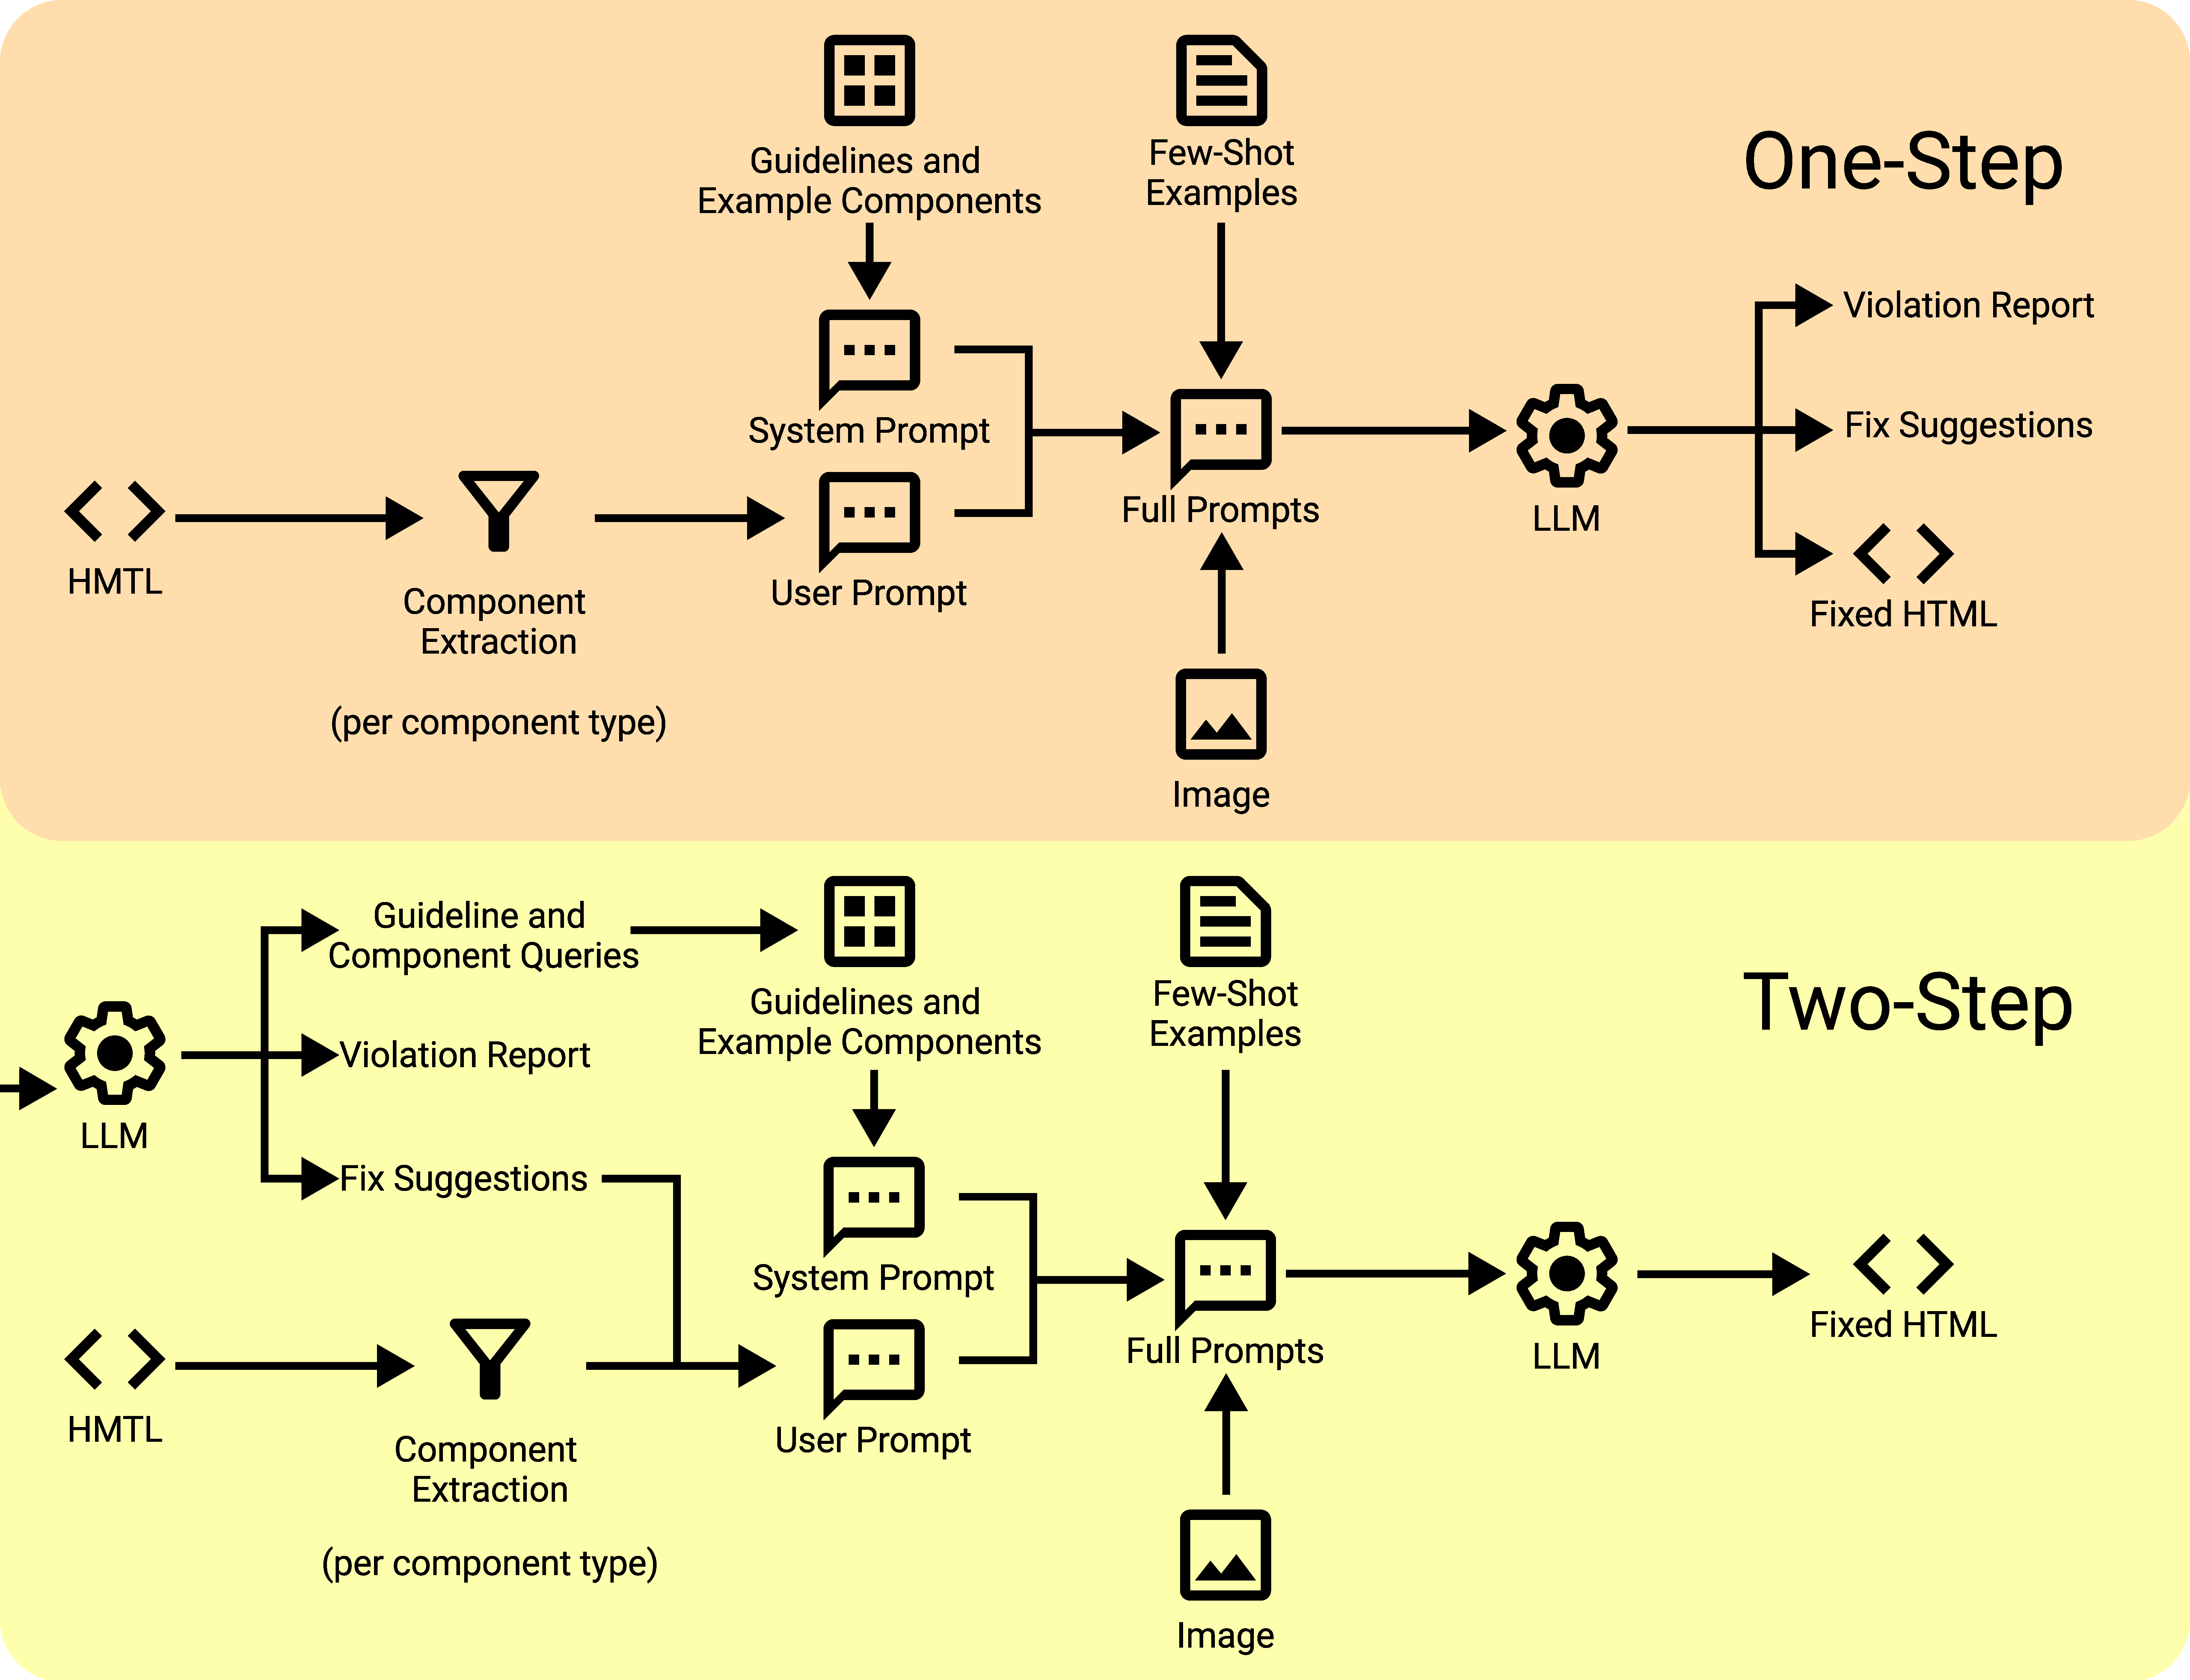
\includegraphics[width=\textwidth]{figures/prompting.pdf}
	\caption{An overview of our two prompting approaches. Note that the first step of the two-step approach looks the same as the one-step approach, so this illustration only includes the second step.}
	\label{fig:prompting}
\end{figure}

Figure \ref{fig:prompting} provides a comprehensive overview of our prompting setup. We perform violation detection, fix suggestion, and change implementation on a per-component-type basis for several reasons: First, most guidelines in Material Design 3 are related to a specific component type. Second, passing every guideline in a prompt could often lead to the prompt exceeding the token limit of GPT-4o. Finally, it has been shown that LLMs tend to perform better when their tasks are split up into more granular steps \cite{khot_decomposed_2023}. The structure of the prompts is the same for every component type: First, the LLM is sent a system prompt containing information about its role and general task, and some instructions on how it should behave. The general guidelines, component type descriptions, component-type specific guidelines, and example implementations from Section~\ref{sec:dataset} are then appended to the system prompt. Next, the LLM is sent a user prompt that explains which component type is being examined and specifies the response format.

There are four different ways the code for the relevant component instances can be extracted: The first method is to extract only the relevant component type's instances and passing them as a list. This approach results in the smallest amount of tokens being sent to the model. However, for many component types, it will likely exclude context that is important to evaluate some guidelines. Thus, the second approach is to locate the component instances, but pass their parent containers to the model, making sure containers that contain multiple instances are passed only once. This gives the model more context to work with. The third approach is the most straightforward one: Simply passing the entire HTML code for the design to the model. However, this approach has two drawbacks: First, complex designs can result in very long HTML files that do not fit into the context window of GPT-4o. Second, for most component types this will include a lot of superfluous information which will at best not be regarded by the model and at worst lead to worse results, as irrelevant code passages can be misinterpreted by the model. The fourth and final approach introduces another step before the actual prompt is created: After using one of the three other approaches, the model is first asked to generate natural-language descriptions of the component instances, including hypotheses about their purposes. After some preliminary tests, we chose to use the following strategy for deciding which extraction method to use when: The full-code method is never used due to the aforementioned drawbacks. We also do not use the description-based method, as it did not seem to improve results during our preliminary tests and increased the amount of needed input and output tokens by a substantial amount. The other two approaches are used depending on which component type is being checked. Larger component types that are less influenced by their surroundings, like navigation bars or top app bars, are extracted using the first method, while smaller components that exist in a larger context, like buttons or checkboxes, are extracted using the second method.

The extracted component instances are appended to the user prompt. Finally, the exported image is also passed to the model in a separate user prompt. The specific instructions in the first user prompt depend on the chosen high-level approach, of which there are two. We refer to the first approach as \emph{one-step}, because it combines the identification and fixing of changes into a single step. Using this approach, the model is asked to describe any issues it found, what it would do to fix these issues, and to provide implementations for these fixes. The second high-level approach is called \emph{two-step}, because it splits up the issue identification and fixing into two prompts. When using this approach, we ask the model to first identify issues and to suggest changes to fix them. The suggestions are then fed back into the model in a second prompt with a request to actually implement them. In the first prompt, the model is also given the opportunity to provide queries for two indexes: One containing every guideline for every component, and one containing all example component implementations. These indexes were created using \texttt{pyterrier}~\cite{pyterrier2020ictir}. The queries are used to retrieve some guidelines and examples from the indexes, which are also appended to the second prompt. This is useful in cases where the model needs to replace an incorrectly used component with one of a different type, for example. 

The response format we ask the model to use is a JSON dictionary, with an entry for each part of the model's answer. The specific contents depend on the chosen high-level method. When using the one-step method, the dictionary contains these entries:
\begin{itemize}
	\item \emph{violations}, a list of natural-language descriptions of issues detected by the model.
	\item \emph{changes}, a list of natural-language descriptions of changes the model suggests to fix the detected issues.
	\item \emph{changed\_components}, a list of HTML components that the model applied changes to.
	\item \emph{deleted\_components}, a list of HTML components that the model wants to remove from the design.
	\item \emph{new\_components}, a list of HTML components that the model wants to insert into the design, each paired with the ID of the element they are to be inserted into.
\end{itemize}

When using the two-step method, the first response contains \emph{violations} and \emph{changes}, and the two new entries \emph{guideline\_request} and \emph{example\_request}, each containing a query for one of the two retrieval indexes. The second response consists of \emph{changed\_components}, \emph{deleted\_components}, and \emph{new\_components}, which contain the same information as in the one-step approach.

We use \texttt{BeautifulSoup}~\cite{noauthor_beautiful_nodate-1} to insert code generated by the model into the HTML file. We parse the model's response using the \texttt{ast} python module \cite{noauthor_ast_nodate}. For the changed components, we use the ID of each component in the list to locate it in the HTML code and replace it with its adjusted version. For the deleted components, the process works analogously. To insert new components, we locate their intended parents using the IDs in the list and insert them as a new child. We also created sets of one to three few-shot examples for every component type using our data set. The few-shot examples have the same structure as new prompts, but also include pre-written answers from the LLM (passed as assistant prompts) and are passed to the model after the system prompt, which is sent only once. For the two-step approach, both prompts include few-shot examples. We created 51 few-shot examples in total, 44 of them using screens from our data set that we manipulated in some way to violate guidelines, and 7 using unmanipulated screens as examples where no changes are necessary. We will show some few-shot examples in the following: 

Figure~\ref{fig:fs_1} shows a few-shot example for the floating action button (FAB) component type, which uses a screen based on \emph{Tricount} \cite{noauthor_tricount_nodate}, a popular expense-tracking app. On the left, which is the incorrect version that is used to create the prompts, the FAB is quite small and placed in the middle of the screen. This violates two guidelines: First, small FABs are intended to be used when a screen contains more than one FAB, in order to not clutter the screen and communicate which action is the most important. Second, FABs should be placed in the bottom right corner of the screens so users can easily reach them with one hand using their thumb. On the right, which is the fixed version produced by our pre-written response, the FAB has the standard size and is located in the bottom right of the screen. 

\begin{figure}[H]
	\centering
	\includegraphics[width=.56\textwidth]{figures/few_shot_1.png}
	\caption{A few-shot example based on the expense-tracking app \emph{Tricount}. In the version on the left, the FAB is small and located in the middle of the screen. In the version on the right, it has been replaced with a larger FAB placed in the bottom right corner.}
	\label{fig:fs_1}
\end{figure}

\begin{figure}[H]
	\centering
	\includegraphics[width=.56\textwidth]{figures/few_shot_2.png}
	\caption{A few-shot example based on the messaging app \emph{WhatsApp}. In the version on the left, common buttons are used to filter search results. In the version on the right, they have been replaced with chips.}
	\label{fig:fs_2}
\end{figure}

\begin{figure}[H]
	\centering
	\includegraphics[width=.56\textwidth]{figures/few_shot_3.png}
	\caption{A few-shot example based on the fitness tracking app \emph{adidas Running}. In the version on the left, labels are used inconsistently in the navigation bar. In the version on the right, all destinations are labeled.}
	\label{fig:fs_3}
\end{figure}

Figure~\ref{fig:fs_2} shows a few-shot example for the common button component type. It uses a screen inspired by the messaging app {\emph{WhatsApp}} \cite{noauthor_whatsapp_nodate}, in which the buttons are used to select various filter options for search results (left). This is not an action that buttons are intended to be used for in Material Design. Chips should be used in their place, as shown in the fixed version (right). 

Figure~\ref{fig:fs_3} shows a few-shot example for the navigation bar component type. It uses a screen inspired by the fitness tracking app \emph{adidas Running} \cite{runtastic_adidas_nodate}. In the incorrect version (left), two of the five destinations in the navigation bar are not labeled, while the three others are. This inconsistency violates Material Design guidelines and is fixed in the correct version (right). 

\begin{figure}[H]
	\centering
	\includegraphics[width=.56\textwidth]{figures/few_shot_4.png}
	\caption{A few-shot example based on the food delivery app \emph{Grubhub}. In the version on the left, checkboxes are used to select an option from a list of mutually exclusive options. In the version on the right, radio buttons are used instead.}
	\label{fig:fs_4}
\end{figure}

Figure~\ref{fig:fs_4} shows a few-shot example for the checkbox component type. It uses a screen inspired by the food delivery app \emph{Grubhub} \cite{noauthor_food_nodate} (known as \emph{Lieferando} in Germany). The incorrect version (left) uses checkboxes to select the sorting of search results, which does not make sense, since multiple checkboxes can be selected at the same time. In the correct version (right), they have been replaced with radio buttons.

\chapter{Evaluation}\label{cha:eval}

We conducted two user studies to evaluate our approach. The first was used to create a test set to evaluate issue identification on and is explained in Section~\ref{sec:ident}, and the second used the results of the first study to evaluate the change implementation capabilities of our approach, as is detailed in Section~\ref{sec:change}.

\section{Issue Identification}\label{sec:ident}

To create test data for the system, the ideal approach would have been a user study where layperson participants create UI designs on their own. These could then have been analyzed by experts to identify issues present in the designs. For one, this would give insights about which types of errors are more common and should be prioritized by the system. Additionally, the designs could be used to test and improve the system by comparing the issues it identifies (or does not identify) with those pointed out by the experts. However, this was not possible due to a lack of time and access to Material Design experts. Instead, we conducted a different user study to create synthetic test data. During the study, participants were given a brief introduction to Material Design and shown how to use Figma. They were then presented with a selection of example designs in Figma, each accompanied by the guidelines for a specific component type. There were 25 examples in total, one for each component type, although some designs were used multiple times. Next, they were asked to modify each example so that at least one of the accompanying guidelines is violated. Participants indicated what they changed and which guideline they deemed to be violated by their change(s). Four people participated in the study, with two of them creating a manipulated version of all 25 screens, one creating manipulated versions for 18 screens, and one creating manipulated versions for 15 screens. Two of the participants had no previous experience with UI design, one had little experience, and one had some experience. None of them had any previous experience working with Material Design 3. The following are some examples of the changes participants made during the user study.

\begin{figure}[t]
	\centering
	\includegraphics[width=.6\textwidth]{figures/us_ex_1.jpg}
	\caption{A generic "settings" screen containing a switch at the bottom of the image, which lets the user toggle the app's access to mobile data. In the original image (left), the switch is labeled "Download using mobile data". In the manipulated image (right), the label has been replaced with "Mobile Data".}
	\label{fig:us_ex_1}
\end{figure}

In Figure~\ref{fig:us_ex_1}, the original screen contains a switch, which is labeled "Download using mobile data". The participant replaced the label with "Mobile data". According to Material Design 3 guidelines, the label of a switch should explain what happens when it is turned on. While the new description is still concerned with the switch's activated state, it is too vague for the user to clearly understand its purpose, which is a guideline violation.

\begin{figure}[t]
	\centering
	\includegraphics[width=.6\textwidth]{figures/us_ex_2.jpg}
	\caption{A screen from a generic email app that contains a snackbar at the bottom of the screen, informing the user that a message has been moved to the trash. In the manipulated version (right), the snackbar has been duplicated multiple times.}
	\label{fig:us_ex_2}
\end{figure}

In Figure~\ref{fig:us_ex_2}, the original screen contains a snackbar, which informs the user that a message has been moved to the trash. The study participant duplicated the snackbar multiple times, which violates Material Design guidelines, since they state that there should only be one snackbar on the screen at a time. 

In Figure~\ref{fig:us_ex_3}, the original screen, which was inspired the messaging app {\emph{WhatsApp}}, contains two floating action buttons. The participant darkened one of them, making it stand out too little from the background, and added a badge to the other, which is not how badges are intended to be used. 

\begin{figure}[H]
	\centering
	\includegraphics[width=.6\textwidth]{figures/us_ex_3.jpg}
	\caption{A screen inspired by the messaging app \emph{WhatsApp}. The original screen (left) contains two floating action buttons in the bottom right corner. In the manipulated version (right), the larger floating action button had its color changed to one with too little contrast and a badge was added to the smaller floating action button.}
	\label{fig:us_ex_3}
\end{figure}

\begin{figure}[H]
	\centering
	\includegraphics[width=.6\textwidth]{figures/us_ex_4.jpg}
	\caption{A screen from a lifestyle app, inspired by an example on the Material Design website. The original screen (left) contains a bottom sheet. In the manipulated version (right), the sheet contains a carousel.}
	\label{fig:us_ex_4}
\end{figure}

In Figure~\ref{fig:us_ex_4}, the original screen, which was inspired by an example on the Material Design website \cite{noauthor_carousel_nodate}, contains a bottom sheet, letting the user share or bookmark one of the events presented on the screen. The study participant replaced some of the elements in the sheet with a carousel. Carousels are used to present primary content, while bottom sheets should contain secondary content, so this is a guideline violation.

\section{Change Implementation}\label{sec:change}

We also conducted a second survey using the data produced by the user study. We had originally planned to ask participants to evaluate the guidance and fixes produced by the system regarding their usefulness. However, since our quantitative analysis, which we present in Section~\ref{sec:quant}, revealed the precision of the system to be very low, we pivoted the second study to strictly evaluating how well the model was able to make changes to HTML code, regardless of how sensible the suggested changes are. Participants were presented with the guideline violations and change suggestions produced by the model, along with a before-and-after image of the corresponding user interface. They were then asked to judge whether or not the model correctly implemented the suggested changes, independent of them making sense. The survey contained 15 examples created using the one-step method and 15 examples created using the two-step method. It should be noted that the methods are not directly comparable, because the suggestions generated for a given screen and component type are not necessarily the same for each method. 


\chapter{Results}\label{cha:res}

In this chapter, we detail the results of the user studies explained in Chapter~\ref{cha:eval}, performing a quantitative and a qualitative analysis on both. Section~\ref{sec:ident_res} shows the results regarding issue identification, while Section~\ref{sec:change_res} does the same for change implementation. 

\section{Issue Identification}\label{sec:ident_res}

\subsection{Quantitative Analysis}\label{sec:quant}

To evaluate the system on the data created during the study, we exported the altered designs and fed them into the system, once using the one-step method, and once using the two-step method, with a request for every component type contained in each design, including those that were not altered by the participants. To make sure that no data leakage occurred, we skipped over component types whose corresponding few-shot examples included screens from the same app the currently evaluated design belonged to. Running this evaluation on every manipulated screen would have resulted in a very large amount of requests, so we decided to use only the 33 changed designs created by the first two participants for a total of 418 requests to the system, 48 of which contained issues. We annotated the model's responses as follows: If the model did not identify any issues, it was labeled with 0, if there was an issue present and it was correctly identified by the model, it was labeled with 1, and if there was an issue present, but the model pointed out something else, it was labeled with a 2. In the ground truth, cases containing no issues were labeled with a 0 and cases with issues were labeled with a 1.

Table~\ref{tab:userstudy} shows the precision, recall, and f1-score values regarding class 1 for the two approaches. Figure~\ref{fig:conf:sub1} shows the confusion matrix of the one-step method, while Figure~\ref{fig:conf:sub2} shows the confusion matrix of the two-step method. It is apparent that regardless of the method used, the system has a very strong tendency to point out issues, independent of the content of a request. Additionally, even if an issue is actually present, it is often not correctly identified. The performance did not differ much between the two methods, with almost identical precision and recall values. The intersections of true positives (19 screens), false positives (132 screens), and misclassified positives (16 screens) are also quite large, indicating that the issues both methods are good (or bad) at identifying are similar. This is not very surprising, as the information for issue identification given to the model is the same for both methods, and the prompts are also very similar.

\begin{table}
	\begin{center}
		\begin{tabular}{|ccc|ccc|}
			\hline
			\multicolumn{3}{|c|}{One Step} & \multicolumn{3}{c|}{Two Step} \\ \hline
			Precision  & Recall & F1-Score & Precision & Recall & F1-Score \\ \hline
			0.15       & 0.52   & 0.24     & 0.14      & 0.5   & 0.22     \\ \hline
		\end{tabular}
		\caption{User Study Annotation results for both methods.}
		\label{tab:userstudy}
	\end{center}
\end{table}

\begin{figure}[t]
	\centering
	\begin{minipage}{.45\textwidth}
		\centering
		\includegraphics[width=\textwidth]{figures/confusion_matrix_one_step.jpg}
		\captionof{figure}{The confusion matrix for the one-step method.}
		\label{fig:conf:sub1}
	\end{minipage}\hfill
	\begin{minipage}{.45\textwidth}
		\centering
		\includegraphics[width=\textwidth]{figures/confusion_matrix_two_step.jpg}
		\captionof{figure}{The confusion matrix for the two-step method.}
		\label{fig:conf:sub2}
	\end{minipage}
\end{figure}

\subsection{Qualitative Analysis}

Due to the large number of false positives generated by the model, we did not perform an exhaustive categorization of errors. Instead, we looked at a randomly sampled subset and selected some interesting examples that illustrate what the model's mistakes and correct responses generally look like. We will show and discuss these examples in the following, beginning with the one-step method.

\subsubsection{One-Step Method False Positives}

\begin{figure}[t]
	\centering
	\includegraphics[width=.28\textwidth]{figures/fp_ex_os_1.jpg}
	\caption{A screen from a generic email app that was falsely reported by the one-step method to have issues regarding its top app bar.}
	\label{fig:fp_ex_os_1}
\end{figure}

A common theme in the model's errors is misunderstanding of HTML code. For example, Figure~\ref{fig:fp_ex_os_1} shows a screen that was falsely identified as containing an issue regarding the top app bar it contains. The model provided this violation report: "The headline text 'Trash' in the top app bar is not center-aligned, which is required for a small-centered top app bar. The leading icon and trailing icon are not balanced around the headline, causing misalignment.", and suggested these changes: "Ensure that the headline 'Trash' is center-aligned and the leading and trailing icons are balanced around it. Adjust the positions of the leading and trailing icons to achieve this." However, it is apparent that the headline is already centered in the original screen, and the trailing and leading icons have the same horizontal margins. A factor that might play a role in this mistake is that text content in Figma usually has bounds that do not define the actual space taken up by the text, but rather the space it \emph{can} take up before being cropped or creating a new line. The placement of the text is then handled through its alignment settings. This is mirrored in our HTML-parsed version: The bounds of the headline container extend left and right to 6 pixels away from each icon, and the text placement is handled by setting the \texttt{justify-content} style attribute to \texttt{center}. Perhaps the model was not able to correctly understand this, causing it to claim the headline is not centered. This misclassification is still a bit surprising, since the headline is implemented the same way in the component examples and few-shot examples given to the model, and the image clearly shows that the headline is centered. 

\begin{figure}[t]
	\centering
	\includegraphics[width=.28\textwidth]{figures/fp_ex_os_3.jpg}
	\caption{A screen inspired by an example from the Material Design website that was falsely reported by the one-step method to have issues regarding the FAB it contains.}
	\label{fig:fp_ex_os_3}
\end{figure}

Another example of misunderstood HTML code is shown in Figure~\ref{fig:fp_ex_os_3}, which shows a screen inspired by an example on the Material Design website \cite{noauthor_bottom_nodate} where the model reported an issue regarding the FAB, which is contained in a bottom app bar. It generated this violation report: "1. Positioning issue: The FAB is located near the top right of the screen. According to Material Design guidelines, FABs should be placed in the bottom right corner to be easily accessible using thumbs. This violation is quite severe because it affects the usability and accessibility of the FAB. 2. Overlapping issue: The FAB is placed in a position where it might overlap with other content, making it difficult for users to distinguish interactable areas. This violation is moderately severe because it can lead to confusion about the interactable areas and impede the visibility of other content." Here, the model was unable to understand the relationship between the FAB's position and its parent's position. Since the FAB is contained within a bottom app bar, it has a small \texttt{top} value, but the bottom app bar is placed at the bottom of the screen. This is also apparent in the image. This connection was too complex for the model to grasp, which claims that the FAB is located near the top right of the screen. 

\begin{figure}[t]
	\centering
	\includegraphics[width=.28\textwidth]{figures/fp_ex_os_2.jpg}
	\caption{A screen from a generic shopping app that was falsely reported by the one-step method to have issues regarding its navigation bar.}
	\label{fig:fp_ex_os_2}
\end{figure}

The model also tends to ignore parts of the information provided to it. For example, Figure~\ref{fig:fp_ex_os_2} shows a screen which the model reported to have an issue regarding its navigation bar, with this violation report: "The navigation bar contains four icons, but one of the icons (the house icon) is not highlighted to indicate the current active screen. This can cause confusion for users as they may not easily identify the current screen they are on." It suggested these changes: "Highlight the active icon (house icon) to indicate the current active screen." As the image shows, one of the icons in the navigation bar is already highlighted (the search icon). The most likely reason for this behavior we could come up with is the example implementations shown to the model, since the first destination is marked as active in all of them. This is not the case in the few-shot examples, however, so the model's misjudgment could be caused by other factors like hallucinations as well.

\begin{figure}[H]
	\centering
	\includegraphics[width=.28\textwidth]{figures/fp_ex_os_4.jpg}
	\caption{A screen inspired by the messaging app \emph{WhatsApp} that was falsely reported by the one-step method to have issues regarding the icon buttons it contains.}
	\label{fig:fp_ex_os_4}
\end{figure}

\begin{figure}[H]
	\centering
	\includegraphics[width=.28\textwidth]{figures/fp_ex_os_5.jpg}
	\caption{A screen from a generic email app that was falsely reported by the one-step method to have issues regarding the bottom app bar it contains.}
	\label{fig:fp_ex_os_5}
\end{figure}


In some cases, the model also struggles with correctly identifying component types: Figure~\ref{fig:fp_ex_os_4} shows a screen that was reported to contain an issue regarding the icon buttons it contains. The model returned this violation report: "1. Inconsistent Icon Button Styles: The icon button for adding a new channel uses a standard style while the other icon buttons use different styles. For consistency and to clearly communicate their importance, the icon buttons should use the same style. (Severity: High)", along with these change suggestions: "1. Change the style of the 'add new channel' icon button to 'tonal' to match the other icon buttons." Looking at the screen, the model's claim is not true, since the buttons using the 'tonal' style are not icon buttons, but common buttons. The model was not able to make this distinction. 

Sometimes, the model's guidance includes logical fallacies. For example, Figure~\ref{fig:fp_ex_os_5} shows a screen that the model reported to exhibit issues regarding its bottom app bar, providing this violation report: "1. The bottom app bar contains only two icons and an FAB. According to Material Design 3 guidelines, bottom app bars should contain up to 4 icon buttons and an FAB. 2. The snackbars are covering the bottom app bar, which should not happen as per the guidelines." and these change suggestions: "1. Add one more icon button to the bottom app bar to make it a total of three icon buttons. 2. Adjust the position of the snackbars so they appear above the bottom app bar." The model presents two correct facts: The bottom app bar does contain two icons and the guidelines do state that bottom app bars can contain up to four icons. However, the conclusion the model draws from this is nonsensical. The second claim is another example of the model making incorrect statements.

\subsubsection{One-Step Method True Positives}

We also examined the true positive cases to get an idea of which types of issues the model was able to identify well. The following are some examples of true positives produced by the one-step method. 

Figure~\ref{fig:tp_ex_os_1} shows a screen that was inspired by the video streaming app \emph{Amazon Prime Video} \cite{noauthor_amazon_nodate} that contains a tab component. One of the tabs has an excessively long label, which was identified by the model in this violation report: "The fourth tab label ('Sports and other non Movie and non Series things') is too long and gets truncated, which makes it ambiguous and hard to read." Strictly text-related issues like this one are ones the model generally seems to perform well on, perhaps unsurprisingly. 

\begin{figure}[H]
	\centering
	\includegraphics[width=.28\textwidth]{figures/tp_ex_os_1.jpg}
	\caption{A screen inspired by the video streaming app \emph{Amazon Prime Video} where the one-step method correctly identified an issue regarding the tabs it contains.}
	\label{fig:tp_ex_os_1}
\end{figure}

It seems the model was also able to relatively accurately identify cases where components were changed too much from their standard implementation. For example, Figure~\ref{fig:tp_ex_os_2} shows a screen containing a menu that was heavily modified. The model identified this, producing this violation report: "1. Missing Text Content: The menu items do not contain any text, which makes them ambiguous and not user-friendly. According to Material Design 3 guidelines, information should be succinct, unambiguous, and not repetitive. 2. Inconsistent Background Colors: The background colors of the menu items are inconsistent, which can confuse users and disrupt the visual hierarchy."

\begin{figure}[H]
	\centering
	\includegraphics[width=.28\textwidth]{figures/tp_ex_os_2.jpg}
	\caption{A screen from a generic shopping app where the one-step method correctly identified an issue regarding the menu it contains.}
	\label{fig:tp_ex_os_2}
\end{figure}

\begin{figure}[H]
	\centering
	\includegraphics[width=.28\textwidth]{figures/tp_ex_os_3.jpg}
	\caption{A screen from a generic email app where the one-step method correctly identified an issue regarding the snackbars it contains.}
	\label{fig:tp_ex_os_3}
\end{figure}

Finally, there are some guidelines that, while still requiring some understanding of a component's purpose, are not very complicated, which the model was able to apply relatively well. Figure~\ref{fig:tp_ex_os_3} shows an example of this. The screen contains multiple snackbars, while the guidelines state that there can only be one snackbar on the screen at a time. The model produced the following violation report: "1. Multiple snackbars are displayed at the same time, which violates the guideline that only one snackbar may be displayed at a time. 2. Snackbars should be placed above any navigation elements and should not obstruct other UI components.", correctly identifying the issue, although the second point is not necessarily correct.

\subsubsection{Two-Step Method False Positives}

We also examined a sample of the false positives generated by the two-step method. In general, these mistakes were similar to those generated by the one-step method.

Figure~\ref{fig:fp_ex_ts_1} shows a screen that was inspired by the social media app \emph{reddit} \cite{noauthor_reddit_nodate} containing a top app bar with two trailing icons. The model claims it contains three, however, as mentioned in its violation report: "The top app bar contains three trailing icons. According to the Material Design 3 Guidelines, the right side of a top app bar should have at most three icon buttons. If more actions need to be accessible, the third icon should be a 'more' icon (three vertical dots) and open an overflow menu." The cause of this mistake might be the names of the trailing icons. The top app bar component from the Material Design kit names the trailing icons from left to right, regardless of their visibility, so the two trailing icons on the screen are named \texttt{trailing-icon-2} and \texttt{trailing-icon-3}. Regardless, even if the top app bar did contain three icons, the model's guidance would be incorrect. As it mentions itself, three trailing icons would not be an issue.

\begin{figure}[H]
	\centering
	\includegraphics[width=.28\textwidth]{figures/fp_ex_ts_1.jpg}
	\caption{A screen inspired by the social media app \emph{reddit} where the two-step method falsely pointed out an issue regarding the top app bar it contains.}
	\label{fig:fp_ex_ts_1}
\end{figure}

\begin{figure}[H]
	\centering
	\includegraphics[width=.28\textwidth]{figures/fp_ex_ts_2.jpg}
	\caption{A screen from a generic email app where the two-step method falsely pointed out an issue regarding the bottom app bar it contains.}
	\label{fig:fp_ex_ts_2}
\end{figure}

Figure~\ref{fig:fp_ex_ts_2} shows a screen containing a bottom app bar with two icons and an FAB. The model generated this violation report: "1. The bottom app bar contains only two icon buttons and an FAB. The bottom app bar should contain 2 to 5 actions. This is a minor violation as the FAB is considered an action. 2. The FAB is placed at the right end of the bottom app bar, which could be inconsistent with the typical placement of the FAB in Material Design guidelines." The first point is another example of the model not understanding numeral guidelines, and the second point seems to be a hallucination, as FABs are always placed on the right side of bottom app bars.

Figure~\ref{fig:fp_ex_ts_3} shows a screen containing a list, for which the model generated the following violation report:  "1. Inconsistent Leading Element Sizes: The leading elements (monograms) have a height of 40px but are placed in containers with a height of 64px. This can create visual inconsistency. (Severity: Medium), 2. Trailing-supporting-text Positioning: The trailing-supporting-text elements have varying left positions, which can disrupt visual alignment and consistency across list items. (Severity: Medium)". The statement from the first point is correct, but the claim of visual inconsistency is untrue, as can be seen from the image. The second point is another case of the model not fully understanding the HTML code. The trailing supporting texts have varying \texttt{left} values, but this is caused by their varying lengths and actually serves to keep them aligned to the right side of the list. 

\begin{figure}[H]
	\centering
	\includegraphics[width=.28\textwidth]{figures/fp_ex_ts_3.jpg}
	\caption{A screen from a generic email app where the two-step method falsely pointed out an issue regarding the list it contains.}
	\label{fig:fp_ex_ts_3}
\end{figure}

Figure~\ref{fig:fp_ex_ts_4} shows a screen containing a navigation bar, for which the model generated the following violation report: "The navigation bar contains icons only, without any labels. According to Material Design 3 guidelines, if one destination in a navigation bar is labeled, all destinations should be labeled. This can cause inconsistency and confusion for users. The color contrast between the icons and the background in the navigation bar is low, which may affect readability and accessibility. Icons should have sufficient contrast against their background to ensure they are easily visible." The second point could be argued about, but since the colors for the bar and icons were created using the Material Theme Builder, we assume that they meet accessibility requirements. In the first point, the model once again contradicts itself. The guideline it refers to is correct, but it does not apply, since none of the destinations are labeled, which is perfectly adherent to the guidelines. 

\begin{figure}[t]
	\centering
	\includegraphics[width=.28\textwidth]{figures/fp_ex_ts_4.jpg}
	\caption{A screen inspired by the social media app \emph{Instagram} where the two-step method falsely pointed out an issue regarding the navigation bar it contains.}
	\label{fig:fp_ex_ts_4}
\end{figure}

Figure~\ref{fig:fp_ex_ts_5} shows a screen containing some radio buttons, for which the model generated the following violation report: "1. The radio buttons are too close to each other, making it difficult for users to distinguish between them. 2. The radio buttons do not have a preselected option, which is necessary for clear user interaction." Since the list items are of a standard size, the distance between the buttons should not be an issue, as their bounding boxes do not overlap. The claim that there is no preselected option seems to be another hallucination, since there clearly is one. 

\begin{figure}[t]
	\centering
	\includegraphics[width=.28\textwidth]{figures/fp_ex_ts_5.jpg}
	\caption{A generic "settings" screen where the two-step method falsely pointed out an issue regarding the radio buttons it contains.}
	\label{fig:fp_ex_ts_5}
\end{figure}

\subsubsection{Two-Step Method True Positives}

As mentioned in the quantitative analysis, the examples the two-step method performed well on were similar to those the one-step method worked well on. The following are some examples of true positives produced by the two-step method.

The two-step method also recognized when components were modified from their original implementations too much. For example, Figure~\ref{fig:tp_ex_ts_1} shows a screen inspired by the social media app \emph{reddit}. It contains a badge in its navigation bar, which is white, making it hard to see against the background color of the bar. The model identified this in the following violation report: "The badge background color (\#FFFFFFFF) is white, which might not provide enough contrast with the icon or its surroundings, especially in light themes. This can make the badge difficult to notice. According to the Material Design 3 Guidelines, badges should have a contrasting color that sticks out from the icon and its surroundings. The badge text color (\#506352FF) is a muted green-gray color, which might not provide sufficient contrast against the white background of the badge. This can make the text hard to read." While the second point is not necessarily true, the reasoning for the first violation is sound. 

\begin{figure}[H]
	\centering
	\includegraphics[width=.28\textwidth]{figures/tp_ex_ts_1.jpg}
	\caption{A screen inspired by the social media app \emph{reddit} where the two-step method correctly identified an issue regarding the badge it contains.}
	\label{fig:tp_ex_ts_1}
\end{figure}

\begin{figure}[H]
	\centering
	\includegraphics[width=.28\textwidth]{figures/tp_ex_ts_2.jpg}
	\caption{A screen from a generic email app where the two-step method correctly identified an issue regarding the dialog it contains.}
	\label{fig:tp_ex_ts_2}
\end{figure}

Like the one-step method, the two-step method also handled text-based issues well, as exemplified in Figure~\ref{fig:tp_ex_ts_2}. It shows a screen containing a dialog, with the confirmation button simply labeled "Ok". This is too vague, as the model points out in its violation report: "1. The primary button label 'Ok' is vague and does not clearly describe the action. 2. The secondary button label 'Cancel' is acceptable but could be more descriptive."

\begin{figure}[H]
	\centering
	\includegraphics[width=.28\textwidth]{figures/tp_ex_ts_3.jpg}
	\caption{A screen inspired by an example on the Material Design website where the two-step method correctly identified an issue regarding the bottom sheet it contains.}
	\label{fig:tp_ex_ts_3}
\end{figure}

While both methods generally struggled with violations requiring a deeper understanding of UI semantics, there were some cases where they accomplished this well, for example in Figure~\ref{fig:tp_ex_ts_3}, which contains a bottom sheet that in turn contains a carousel. Bottom sheets are intended to display secondary content and carousels usually serve as main content, so this is a violation. The model produced this violation report: "1. Bottom Sheet Content: The bottom sheet contains a carousel, which is not typically secondary content. Bottom sheets should contain secondary content, not the main content of the app. This is a moderate violation because it affects the clarity of the app's content hierarchy. 2. Bottom Sheet Height: The bottom sheet appears to be too tall. Bottom sheets should not cover too much of the screen initially. This is a minor violation as it affects usability slightly.", correctly identifying this issue.

\subsection{Summary}

Our quantitative analysis produced two main insights: Both methods performed very similarly regarding issue identification, and both had a very strong tendency to produce false positives. Our qualitative analysis revealed some possible causes for this: First of all, the model struggles with the relatively complex structure of our HTML code, frequently misinterpreting where components are placed. It also struggled with logical reasoning. Additionally, the model frequently hallucinates issues. The strengths of the model are analyzing text-based issues, recognizing when components are modified too heavily, and guidelines that are very straightforward. 

\section{Change Implementation}\label{sec:change_res}

\subsection{Quantitative Analysis}

Three main types of errors can occur regarding change implementation when using our prompting approaches: \emph{Prompt errors} that occur when the length of a prompt exceeds the context window of GPT-4o (128000 tokens), \emph{JSON errors} that occur when the output produced by the model can not be parsed as JSON data correctly (caused by incorrect syntax or an output that is too long and gets truncated), and \emph{HTML errors} that occur when parts of the output produced by the model contain errors in respect to the HTML code (usually use of non-existent component IDs when inserting new components). How often these errors occur per method is illustrated in Figure~\ref{fig:error_counts}. Note that if one type of error occurs, the next type(s) of errors cannot occur, since the process cannot continue from that point on. The biggest discrepancy in error counts between the two methods can be seen when looking at the prompt errors, where the one-step method did not produce any errors, while the two-step method produced 57~errors. This is caused by the two-step method generating very long prompts for component types that typically use more code (like lists or navigation bars). This did not occur during our tests before the user study, which is why we did not consider it, but mitigating this type of error would not be very complicated. Looking at the cases where the model actually had a chance to respond to the prompts, the one-step method produces more JSON code that cannot be parsed than the two-step method. This likely has the same cause as the high rate of prompt errors for the two-step method: When the model creates a fix for a more complex component type, it is more likely to reach the limit of tokens it can produce before finishing the code, resulting in a JSON file that cannot be parsed correctly. For the final error type, the two methods do not differ much. 

\begin{figure}[t]
	\centering
	\includegraphics[width=\textwidth]{figures/error_counts.png}
	\caption{The number of errors per error type that occurred for each method when evaluating the system on the user study.}
	\label{fig:error_counts}
\end{figure}

\pagebreak 

Three people participated in this study. One participant (participant 2) had little experience with UI design and Material Design 3, one (participant 0) had some experience with both, and one had a lot of experience with both (participant 1). None of these participants took part in the previous user study. Figure~\ref{fig:change_imp} details their responses to the survey, along with an aggregate rating created through majority voting. For the one-step method, the participants deemed $47\%$ of the changes to be implemented correctly. However, the inter-rater agreement was relatively low, with a Fleiss' Kappa value of $0.1$. For the two-step method, only $20\%$ of the changes were deemed to be implemented correctly by the participants. Inter-rater agreement was extremely low, however, with a value of $-0.02$, which indicates that the participants had opposing views on many examples. Looking at each participant's isolated answers further illustrates their disagreement. Participant 0 actually annotated the same amount ($66\%$) of change implementations to be correct for both methods, and participant 2 also evaluated both methods relatively similarly. Participant 1 had the biggest change in opinion between the two methods, rating the two-step method much lower than the one-step method. The high degree of disagreement between participants could imply that we did not explain the annotation task well enough, but it also illustrates the complicated nature of the model's task.

\begin{figure}[t]
	\centering
	\includegraphics[width=\textwidth]{figures/change_implementation_survey_results.png}
	\caption{The ratio of changes each participant deemed to be implemented correctly for each method.}
	\label{fig:change_imp}
\end{figure}

\subsection{Qualitative Analysis}

As noted above, inter-rater agreement was extremely low, so we will only include examples that all participants agreed on in this qualitative analysis. To make the differences between the unchanged and changed versions more apparent, we marked the areas that were modified in every Figure with red rectangles.

\subsubsection{One-step incorrectly implemented changes}

We will begin by presenting examples where the one-step method was not successful in performing the changes it described.

Figure~\ref{fig:change_bad_ex_os_1} shows another of the many examples where the model did not understand the hierarchical structure of our HTML code, as it claims the FAB the screen contains is located in the top right of the screen, leading it to suggest these changes: "1. Reposition the FAB to the bottom right corner of the screen to improve accessibility and adherence to the guidelines. Ensure it does not overlap with any navigation or bottom app bars." In the "fixed" version, the FAB has completely disappeared. Looking at the code generated by the model reveals that it has not been removed, but that the misinterpretation regarding its position carried over, with its position being changed to a \texttt{left} value of 340 and a \texttt{top} value of 730. Since the bottom app bar containing the FAB is already at the bottom of the screen, this moves the FAB far outside the bounds of the image. Manually moving the "fixed" FAB one step up in the hierarchy so that it is no longer contained in the bottom app bar results in it ending up in the same place as before.

\begin{figure}[t]
	\centering
	\includegraphics[width=.56\textwidth]{figures/change_bad_ex_os_1.jpg}
	\caption{A screen where the model falsely identified an issue with the FAB and suggested moving it (left). In the "fixed" version (right), the FAB was moved outside of the frame.}
	\label{fig:change_bad_ex_os_1}
\end{figure}

Figure~\ref{fig:change_bad_ex_os_2} shows a screen containing a list that the model deemed to be containing too few dividers, suggesting these changes: "1. Add a divider between "Language" and the radio buttons. 2. Add a divider between "Email settings" and the switch. 3. Add a divider between the "Receive emails" switch and the checkboxes." As the image shows, the "fixed" version is the exact same as the original. An inspection of the code generated by the model reveals the reason for this: The three dividers mentioned by the model are actually correctly implemented, but it did not adjust the height of the list items containing the new dividers accordingly, leading to them being hidden from the user. This continues the pattern of the model struggling to work with more complex parts of HTML code.

\begin{figure}[H]
	\centering
	\includegraphics[width=.56\textwidth]{figures/change_bad_ex_os_2.jpg}
	\caption{A screen where the model suggested adding more dividers (left). The "fixed" version (right) looks the same, because the dividers were not added correctly.}
	\label{fig:change_bad_ex_os_2}
\end{figure}

\subsubsection{One-step correctly implemented changes}

The following are examples of changes the one-step method implemented successfully.

Figure~\ref{fig:change_good_ex_os_1} shows a screen containing some standard icon buttons. The model decided they do not stick out enough and recommended replacing them with filled icon buttons: "Change the 'standard' configuration of the icon buttons to 'filled' for higher emphasis and better visibility." It accomplished this change successfully, which shows that the component examples we provide are useful to the model, at least in some cases.

\begin{figure}[H]
	\centering
	\includegraphics[width=.58\textwidth]{figures/change_good_ex_os_1.jpg}
	\caption{A screen where the model suggested changing the style of the icon buttons to 'filled' (left), and the fixed version (right).}
	\label{fig:change_good_ex_os_1}
\end{figure}

\begin{figure}[H]
	\centering
	\includegraphics[width=.58\textwidth]{figures/change_good_ex_os_2.jpg}
	\caption{A screen containing a dialog for which the model suggested new text (left), and the fixed version (right).}
	\label{fig:change_good_ex_os_2}
\end{figure}

Figure~\ref{fig:change_good_ex_os_2} shows one of the cases where the model correctly identified an issue and also correctly fixed it. The label "Ok" for the confirmation action of the dialog on the screen is too vague, while "Delete" accurately communicates what happens upon confirmation. While also changing the headline of the dialog is not really necessary, the changed version is not harder to understand than the original, so this change is not detrimental. There is a slight mistake in the fixed version, as the "Delete" label gets cut off a bit. The model actually increased the width of the label text element to adjust it for the longer label, but once again struggled with understanding more complicated interactions, as it would have also had to change the \texttt{left} value of the label text to center it and avoid it getting cut off.

\subsubsection{Two-step incorrectly implemented changes}

Next, we will show some examples of changes incorrectly performed by the two-step method.

Figure~\ref{fig:change_bad_ex_ts_1} shows a case that is relatively hard to judge. Regarding the radio buttons the screen contains, the model reported the following issues: "1. The radio buttons are nested within a div with the same top and left positions, which makes them appear as if they are overlapping. This can cause confusion as to which radio button is selected. 2. There is no preselected option for the radio buttons, which is against the guideline that there should always be a preselected option when using radio buttons." The first issue seems to be caused by a misunderstanding of HTML code, while the second might be a hallucination, as there already is a preselected option present. The model suggested these changes: "1. Ensure that the radio buttons are not overlapping by adjusting their top and left positions. 2. Set one of the radio buttons as the preselected option." Since both requirements are actually already fulfilled in the original image, the ideal response would be to change nothing. What the model actually did was move the preselection from the first radio button to the second.

\begin{figure}[H]
	\centering
	\includegraphics[width=.56\textwidth]{figures/change_bad_ex_ts_1.jpg}
	\caption{A screen containing radio buttons, for which the model suggested some non-sensible changes (left). In the "fixed" version, a different radio button is preselected.}
	\label{fig:change_bad_ex_ts_1}
\end{figure}

\begin{figure}[H]
	\centering
	\includegraphics[width=.56\textwidth]{figures/change_bad_ex_ts_2.jpg}
	\caption{A screen containing multiple cards (left). In the "fixed" version (right), the text on the cards has been shortened and the "share" button has been duplicated.}
	\label{fig:change_bad_ex_ts_2}
\end{figure}

For the cards in the original screen in Figure~\ref{fig:change_bad_ex_ts_2}, the model suggested these changes: "Reduce the amount of text in the 'Title' section to make it more succinct and easier to read. Consider breaking up the text into smaller, more digestible chunks or using bullet points. Increase the spacing between the buttons in the 'Actions' section to ensure they are not too close to each other and are easy to interact with. Increase the spacing around the 'Subhead' text in the 'Header' section to make it easier to read and less crowded." The first change was correctly implemented by simply truncating the text. For the second change however, the model did not move or replace the buttons, but instead inserted copies in slightly changed positions without removing the old buttons, pointing to a misunderstanding of the output format. To implement the final change, the model added margins to the subhead elements, which inadvertently lead to the text getting cropped. 


\subsubsection{Two-step correctly implemented changes}

Finally, the following are examples of changes the two-step method was able to perform correctly.

Figure~\ref{fig:change_good_ex_ts_1} shows an example of the model working well with text-only changes, but also demonstrates a certain level of semantic understanding. Regarding the checkboxes on the screen, the model returned these issues and change suggestions: "Violations: 1. The checkboxes in the 'Select all' section and the individual items are correctly used. However, the dialog box that appears when moving items to a folder is not clearly connected to the checkboxes, which may cause confusion for the user. This could be improved by making it more obvious that the action is related to the selected items. Changes: 1. Add a clear visual connection or indication that the dialog box is related to the selected checkboxes. This could be done by highlighting the selected items or adding a brief message in the dialog box that mentions the number of selected items." It implemented the suggestion by simply adding an item count to the dialog's supporting text, which mentions the correct number of selected checkboxes.

Figure~\ref{fig:change_good_ex_ts_2} is another example of text-based changes working well. The model deemed the text on the cards to be too long and suggested these changes: "Move the 'A user has reported you' badge closer to the relevant content it is associated with, such as next to the user's profile picture or name. Reduce the amount of repetitive placeholder text ('Lorem ipsum dolor sit amet...') in the cards to make the content more succinct and easier to scan." The change regarding the badge was not implemented well, with it being moved next to the search icon, but the second change was correctly implemented. 

\begin{figure}[H]
	\centering
	\includegraphics[width=.56\textwidth]{figures/change_good_ex_ts_1.jpg}
	\caption{A screen containing a dialog, for which the model suggested some additional text (left). In the fixed version (right), the new text has been added.}
	\label{fig:change_good_ex_ts_1}
\end{figure}

\begin{figure}[H]
	\centering
	\includegraphics[width=.56\textwidth]{figures/change_good_ex_ts_2.jpg}
	\caption{A screen containing a badge and cards (left). The model suggested moving the badge and truncating the card's titles, as shown in the fixed version (right).}
	\label{fig:change_good_ex_ts_2}
\end{figure}

\subsection{Summary}

Our quantitative analysis regarding change implementation was not very insightful, as the high inter-rater disagreement makes the data hard to work with. Our qualitative analysis of the examples all raters agreed on did produce some insights, however: The issues with working with HTML code that occurred during issue identification carried over to change implementation, leading to half-correct changes that were missing the final clean-up steps to be completed. The strengths of the model were transferring code from the examples it was provided into new screens and working with text, also mirroring some of its strengths regarding issue identification. 

\chapter{Discussion}

In this chapter, we begin by discussing the results of our analyses from Chapter~\ref{cha:res} in relation to our research questions from Section~\ref{sec:rq_intro} in Section~\ref{sec:rq}. We also acknowledge the limitations of our approach and the threats to its validity in Section~\ref{sec:lim} and Section~\ref{sec:threat} respectively.

\section{Research Questions}\label{sec:rq}

\subsection{RQ 1: Are large language models able to understand UI design guidelines? (Issue Identification)}

Since the results produced by both methods regarding issue identification were largely similar, we believe the following insights hold true for both. Judging by the results of our analysis, it seems that LLMs were less capable of dealing with UI design than we initially expected. The quantitative analysis regarding issue identification led to one main insight: GPT-4o has a very strong aversion to replies where it does not report any issues. It is hard to pinpoint the reason for this behavior, as it likely is caused by a multitude of factors. One of these factors might be the RLHF stage of the model's training, as it likely discourages short responses \cite{singhal_long_2024}, which conflicts with what would be ideal for most cases in our scenario. Our qualitative analysis revealed some other insights that help to explain the lackluster performance: While the model is able to generally understand and work with HTML code, the relatively complicated structure of the code generated through our approach seemed to cause some issues. The well-known issue of hallucinations also occurred relatively often. Additionally, the model struggled quite a bit with logical reasoning, especially regarding numerical bounds. While the model did sometimes point to the images it was provided with in its answers, it seems that it was not able to consistently match which parts of the code belonged to which part of the image. Also, some of our descriptions of component types likely were too vague, exemplified by the model's tendency to confuse component types. The model had more success regarding simpler guidelines, so it is also possible that we did not define the more complicated guidelines with enough detail.

\subsection{RQ 2: Are large language models able to modify UIs in a sensible manner? (Change Implementation)}

Regarding fix implementation, the difference in performance between the two methods indicates that the two-step method possibly does not provide enough information for the model to accurately implement fixes, although it is unclear if this lack of information is caused by our prompts or by the suggestions from the first step not being detailed enough. Additionally, the two-step method clearly needs to be made more robust regarding the length of prompts for the second step. In general, however, the results indicate similar problems to the issue identification part: The model struggled to deal with our HTML code much more than we anticipated. It often was able to perform the "first steps" of changes, but failed to deal with the implied "next steps". Relationships between parent and child tags like positions were rarely considered by the model when making changes, leading to strange results. On the other hand, simple, text-based changes were easy for the model to implement. It also seems like the example components we provide to the model were useful, as it was able to replace others with them in some cases.
%html understanding limited, some guidelines too vague, 

\section{Limitations}\label{sec:lim}

The most obvious limitation of our approach are the lackluster results caused by hallucinations, logical reasoning errors, and problems with complex code, as discussed earlier. Additionally, our focus is quite limited, as we examine only mobile UIs developed for smartphones using a specific design system. However, we believe our approach could be adapted for other devices, screen sizes, and design systems. Finally, while we provide an accessible pipeline for all three modules we developed, our system is far from usable for its intended target group, as we require users to export their designs using a specific plug-in and then run the system using the command line. A finished version of our system would have to be integrated into the Figma API and accessible as a plug-in. Another limitation of our approach is that we rely on users not renaming components in order to identify them.

\section{Threats to Validity}\label{sec:threat}

There are a few threats to the validity of our work, the biggest being that no UI design or Material Design experts were involved in our research or development process, which potentially could have led to some mistakes regarding the understanding of guidelines. Additionally, even though our data set is mostly inspired by well-known apps, it was still manually created by only one person, likely introducing some sort of bias. It is also not very large, resulting in relatively small sample sizes for our quantitative analysis. Similarly, the screens produced by our user study were not created in a natural environment and none of the participants had experience with Material Design. The change implementation study also had a low sample size and very low inter-rater agreement, possibly pointing to problems in its setup.

\chapter{Related Work}\label{cha:related}

This chapter will present some papers that are relevant to our work. In Section~\ref{sec:sim}, we present some works that have similar goals to ours and explain how they differ from our approach. Section~\ref{sec:assist} shows UI design assistance systems that are not as close to our work. Finally, Section~\ref{sec:repair} presents LLM-based automated code repair systems, a topic that is related to the change implementation part of our work.

\section{Guideline Violation Detection Systems}\label{sec:sim}

An approach that is close to the one presented in this thesis is proposed by Lu et al. in \cite{lu_ai_2024}. They conducted a workshop with UI designers to elicit their requirements for an artificial intelligence-based UI linting tool. They identified four key requirements designers had for such a system: 
\begin{itemize}
	\item Detected violations should be explained and pointed out in screenshots.
	\item The tool should have a successful completion rate of $90\%$ or more.
	\item The tool should provide a confidence level for its results.
	\item The tool should be able to analyze multiple apps at once.
\end{itemize}

Using these requirements, they prototyped and iterated upon various technical solutions, gathering feedback from designers with every iteration. \pagebreak

Through this process, they identified three main themes of the goals and needs designers had:

\begin{samepage}
	\begin{itemize}
		\item Change suggestions should always correspond to specific system guidelines.
		\item The detection of pixel-level violations should be extremely precise.
		\item Feedback and change suggestions should be clear and well-explained.
	\end{itemize}
\end{samepage}


These insights led to the proposal of a hybrid approach, combining heuristics and AI-based techniques in a pipeline consisting of three modules. Note that Lu et al. only aimed to develop an architecture and did not actually implement their proposed approach.

The first module extracts component-specific information (e.g. height, width, padding, number of sub-elements) from view hierarchies to provide the model with exact, pixel-level information. The second module is used to extract the guidelines that are relevant for a screen from the design system specifications using embedding-based retrieval techniques on a vector database containing all guidelines. The final module combines the information from the two previous modules into a prompt that is passed to an LLM, which then produces natural-language feedback. Their approach has two main differences to our work: First, guidelines that need more context and/or semantic understanding of UI design are ignored in their work, because their target group (experts) likely would not create issues regarding these types of guidelines. Our approach includes these guidelines, as it aims to target inexperienced users. Additionally, their pipeline produces only descriptions and recommendations for issues, while we also attempt to fix the issues automatically.

Duan et al. present a different UI design assistance system that uses LLMs in \cite{duan_generating_2024}. They developed a Figma plug-in that can be used to check UI design mock-ups against various collections of guidelines. Their focus is much wider than that of this thesis: Mockups can be any type of UI (mobile, websites, etc.) and do not have to use a specific design system. Their target group also differs from ours, as they aim to provide assistance to professional developers, not novices. The guidelines they use are also more general, for example the well-known usability heuristics by Nielsen \cite{experience_10_nodate}. Users can also enter their own guidelines or ask any other questions about their design. When a user starts the plug-in's evaluation, a JSON representation of their mockup and the guidelines they selected are passed to an LLM. The response by the model is presented as plain text with some augmentations to help the user work with the guidance provided by the model. Group and component names that are mentioned in the text can be hovered to highlight the corresponding element(s) in the mockup. Additionally, single violations can be dismissed by users, which is given to the LLM as feedback for following evaluation runs. They conducted three studies to evaluate their system: 

The first study aimed to evaluate the model's usefulness. Three design experts were presented with the suggestions generated by the model for 51 unique UIs and asked to rate their accuracy from one to three and their helpfulness from one to five. This study produced favorable results, with $52\%$ of the suggestions being rated accurate, $19\%$ partially accurate, and $29\%$ not accurate. Additionally, $49\%$ were rated helpful or very helpful, $15\%$ moderately helpful, and $36\%$ slightly or not helpful. However, it has to be considered that the inter-rater agreement (Fleiss' Kappa) was relatively low ($0.112$ for the accuracy ratings and $0.100$ for the helpfulness ratings). 

In the second study, twelve design experts were asked to check 12 UIs each against the same guidelines as the model, and then compared their results with those of the model. To calculate performance metrics for this study, the 91 violations identified by the experts along with 9 violations found by GPT that were deemed helpful in the first study and missed by the experts were used as a ground truth set to evaluate the model in terms of precision, recall, and f1-score. The same metrics were computed for each expert and averaged. The results of this study are detailed in Table~\ref{tab:duan}. The model was outperformed quite strongly by the human evaluators in terms of precision ($0.603$ to $0.829$), but achieved a higher recall than them ($0.380$ to $0.336$), resulting in very similar f1-scores ($0.466$ and $0.478$). 

\begin{table}
	\centering
	\begin{tabular}{|ccc|}
		\hline
		\textbf{Metric} & \textbf{GPT-4} & \textbf{Human Evaluators (Avg.)} \\ \hline
		Precision       & 0.603          & 0.829                            \\ \hline
		Recall          & 0.380          & 0.336                              \\ \hline
		F1-Score        & 0.466          & 0.478                            \\ \hline
	\end{tabular}
	\caption{A table detailing the results of the violation identification survey conducted by Duan et al. in \cite{duan_generating_2024}.}
	\label{tab:duan}
\end{table}

The final study aimed to evaluate the model's iterative performance. Twelve different design experts used the system on three UIs each, being asked to once again rate the accuracy and helpfulness of the suggestions, but also to implement the helpful suggestions, and then re-run the model on the adjusted UIs to rate the new suggestions. For two of the three UIs, they performed one round of edits and two rounds of ratings, and for the third, they performed two rounds of edits and three rounds of ratings. Figure~\ref{fig:duan_iter} shows the distribution of ratings per round: The initial accuracy ratings were similar to those from the first study, but declined with each round of ratings, dropping from $52\%$ accurate, $28\%$ partially accurate, and $20\%$ not accurate to $39\%$ accurate, $26\%$ partially accurate, and $35\%$ not accurate. The helpfulness ratings also declined from $47\%$ helpful, $19\%$ moderately helpful, and $34\%$ slightly or not helpful to $33\%$ helpful, $16\%$ moderately helpful, and $51\%$ slightly or not helpful. However, once again, the inter-rater agreement was relatively low ($0.155$ for accuracy and $0.085$ for helpfulness). 

\begin{figure}[H]
	\centering
	\includegraphics[width=\textwidth]{figures/duan_iterative.png}
	\caption{A figure from \cite{duan_generating_2024}, detailing the results of the iterative usage study performed by Duan et al.}
	\label{fig:duan_iter}
\end{figure}

The second and third studies also included a short interview at the end of each session to gather some qualitative inputs. In these interviews, the participants identified various strengths and weaknesses of the system: The LLM was able to identify issues that are more subtle and easy to overlook, like small visual details. It also was successful at identifying text-related issues and reasoning with UI semantics. On the other hand, the LLM tended to apply guidelines too literally and to ignore context which would lead to some guidelines not applying. Its suggestions were also too repetitive and too vague sometimes. Due to being based only on JSON representations, there were also cases where the model claimed that elements overlapped, which was not the case in the actual visual designs. In general, study participants found the tool useful, reasoning that experts are able to recognize and ignore the errors made by the model. However, they also noted that this would not be the case for novices. These qualitative insights mirror some of our findings.

Yang et al. present a tool called \emph{UIS-Hunter} in \cite{yang_dont_2021}. They based their work on the Material Design 2 guidelines, which they compiled into a knowledge base and an example gallery. Similar to Material Design 3, Material Design 2 guidelines are mostly defined in relation to a specific component type. To analyze a UI design, UIS-Hunter requires an image and component metadata (like that contained in rico, for example). These inputs are fed into four extractors, which collect atomic information about the text contained in each component, every component's edges, the icons contained in each component, and the color(s) of each component. The extracted information is then fed into a validator which checks if any guideline (defined as boolean clauses) is violated. Finally, a violation report is generated. The report lists every violated guideline and provides examples from the gallery to assist in fixing the error. The report also contains an image of the UI where the problematic components are highlighted. UIS-Hunter was evaluated on a subset of rico containing 60,756 UIs (with 118,999 instances of relevant components). It reported 12,621 guideline violations, which were manually checked for correctness, resulting in an average precision of $0.81$. Since analyzing every UI for which no violation was reported (of which there were 50,829) was not feasible, the false negative rate was estimated using a sample of 3490 UIs, resulting in a recall of $0.9$ and thus an f1-score of $0.87$. It should be noted that rico UIs do not necessarily use Material Design components, but the component types from the provided metadata can be mapped onto them. Since no violations were found in rico for 26 guidelines, a second evaluation was performed. It was done using a set of example Figma designs for Material Design 2 provided by Google consisting of 413 UIs, to which Yang et al. added 80 manipulated versions that deliberately violate the 26 missing guidelines, resulting in 493 examples. On this set, UIS-Hunter achieved a precision of $0.94$, a recall of $0.95$, and an f1-score of $0.95$. Finally, a user study was conducted to compare the performance of UIS-Hunter to that of human evaluators: Five front-end developers with at least one year of mobile and/or web-app development experience were presented with 40 UIs from rico, 27 of which contained violations and 13 of which did not. They were presented with the 18 guidelines that were relevant to these UIs, including examples, and then asked to inspect them. In this test, the participants achieved an overall average precision of $0.755$ and a recall of $0.719$, indicating that UIS-Hunter outperforms human evaluators. While this approach is overall similar to ours, there are some key differences. Most notably, their work focuses on Material Design 2, while we used the more recently released Material Design 3. While many component types and guidelines are shared between these two design systems, they are not identical, so UIS-Hunter could not be applied to Material Design 3 UIs without some adjustments, which has not been done to the best of our knowledge. Also, while UIS-Hunter provides	 textual descriptions of issues, they are sourced from the example gallery and thus not as case-specific as the reports generated by LLMs our approach provides. Additionally, we also aimed to perform fixes for detected violations, which UIS-Hunter does not. 

\section{Other UI Design Assistance Systems}\label{sec:assist}

In \cite{lee_guicomp_2020}, Lee et al. develop GUIComp, an assistance tool for GUI prototyping, which can be used as an add-on for the browser-based prototyping tool KakaoOven~\cite{oven_corp_ovenappio_2024}. They began their work with a qualitative user study to elicit the requirements novice UI designers have for such a system. Their study had 16 participants, all of which had no previous experience with UI design, but were interested in designing UIs in the future. Participants were tasked with creating a UI design using the standard version of KakaoOven, and then were interviewed to identify which challenges they came across. The study found three main difficulties users ran into: 
\begin{itemize}
	\item They consistently had issues starting out and sought out examples or templates online to get a first idea of what their design could look like.
	\item Participants were unsure about the quality of their designs and found it hard to make choices.
	\item Participants wanted to make sure users noticed important parts of their design, but were not certain about how to accomplish this.
\end{itemize}
These requirements were taken into account when developing GUIComp, which provides three feedback panels to the user, each addressing one of the requirements elicited in the study. Figure~\ref{fig:guicomp} shows what the interface of GUIComp looks like.

\begin{figure}
	\centering
	\includegraphics[width=\textwidth]{figures/GUIComp.png}
	\caption{A figure from \cite{lee_guicomp_2020} which shows the user interface of GUIComp. Panels A1-A3 belong to the base tool (KakaoOven), while the Evaluation (B), Recommendation (C), and Attention (D) panels are added by GUIComp.}
	\label{fig:guicomp}
\end{figure}

The first panel, the Evaluation panel, provides information about the values of the complexity metrics proposed by Riegler and Holzmann \cite{riegler_measuring_2018} (explained in Section~\ref{sec:metrics}), by presenting them in relation to a subset of the rico data set. This gives users an idea of the quality of their design. The second panel, the Recommendation panel, extracts UIs that are similar to the current design from rico using the k-nearest neighbor algorithm on data generated using an autoencoder, along with some randomly chosen UIs, to provide the user with inspiration. Finally, the Attention Panel uses a graphic design importance attention model \cite{bylinskii_learning_2017} to compute a heatmap indicating where potential end users are most likely to look when interacting with the GUI. GUIComp was evaluated in another User Study where 30 participants were asked to design two UIs each, with 15 participants using KakaoOven without GUIComp, and 15 participants using KakaoOven with GUIComp. After completing their task, participants were asked to fill out a questionnaire regarding their experience. The use of KakaoOven with GUIComp was consistently rated as more satisfying, efficient, fun, fulfilling, effective, and comfortable than that of KakaoOven without GUIComp. To evaluate the quality of the designs produced during the study, 26 \emph{Amazon Mechanical Turk} \cite{noauthor_amazon_nodate-1} workers were asked to rate the quality of designs on a 1-10 scale with no additional instructions, and 21 other workers were asked to rate the quality of the designs on a 1-10 scale while being provided with the complexity metric values to guide their assessment. In both cases, the designs created using GUIComp were consistently rated higher than those created without GUIComp. To gauge how users actually interacted with GUIComp's panels, eye-tracking data was recorded for 9 participants. The tracking data showed that users often looked at the recommendation panel in the earlier phases of the design process and then began looking more at the evaluation and attention panels later on, indicating that the panels were being used as intended. In terms of limitations, participants mentioned that they would have liked to be provided with more reasoning for the feedback they were given by GUIComp, and some noted that they would find automated correction of errors useful. Additionally, some users ignored feedback they personally disagreed with, possibly caused by the lack of reasoning. We took some inspiration from GUIComp for our work, most notably the metrics used in the evaluation panel, and we believe that our approach tackles some of the limitations of GUIComp by providing more specific guidance and textual feedback.


In \cite{kolthoff_data-driven_2023}, Kolthoff et al. develop \emph{RaWi}, which is a system for UI prototyping that assists designers by letting them retrieve UI examples from a large data set based on natural language queries. The retrieved examples are editable, so they can be used as templates in their entirety, or specific components can be reused for the user's design. To evaluate their approach, they created a gold standard set of queries and relevant screens using \emph{Amazon Mechanical Turk}. The gold standard was used to compare baseline information retrieval approaches, automatic-query-expansion-based approaches, and BERT-based approaches. They found that the BERT-based approaches achieved the best performance on the gold standard. They also performed a user study which indicated that RaWi increased the productiveness of UI prototyping. The user study participants also generally found RaWi to have a high level of usability. 

\section{LLM-based Program Repair Systems}\label{sec:repair}
	
Bouzenia et al. present \emph{RepairAgent} in \cite{bouzenia_repairagent_2024}. It gives an LLM (GPT-3.5) access to a selection of tools for Java code repair using a middleware that orchestrates communications between the LLM and the tools in an iterative manner. Fixing a bug consists of multiple steps, in each of which the LLM is prompted by the middleware with a dynamically changing prompt. The prompt consists of a static and a dynamic part: The static part which contains information about the role and goals of the LLM, some guidelines and an output specification. The dynamic part contains a description of the current state of the fixing process, a list of the tools available in the current step, the information gathered in previous steps, and the command that was executed in the previous step and its result. The middleware adjusts the state and available tools based on a finite state machine (FSM), which guides the LLM between the states \emph{Understand the bug}, \emph{Collect information to fix the bug}, \emph{Try to fix the bug}, and \emph{Done}. The tools available to the LLM are grouped into four categories:
\begin{itemize}
	\item \emph{Read and extract code}, which includes functions to read a selection of lines of code, extract classes and methods from a file, extract a specific method from a file, and to extract the code of failing unit tests. 
	\item \emph{Search and generate code}, which includes functions to scan the files in a project for some keywords, to find API calls similar to a code snippet including an API call, and asking a second LLM to generate the body of a method based on the code preceding it.
	\item \emph{Testing and patching}, which includes functions to run the tests included in a project, to retrieve fault localization information, and to apply a fix to the code and run the project's tests.
	\item \emph{Control}, which includes methods to move the FSM into the \emph{Collect information to fix the bug} state, to move the FSM into the \emph{Understand the bug} state, and to declare that the goal has been accomplished.
\end{itemize}

The process is stopped when the bug is fixed or when a predefined budget runs out. RepairAgent was evaluated on the Defects4J 1.2 and 2.0 data sets \cite{just_defects4j_2014}, which contain 395 and 440 bugs from real Java projects respectively. It was able to fix 164 bugs, which is comparable to state-of-the-art approaches. Notably, RepairAgent was able to fix more bugs requiring more than one line of fixes than the baseline approaches. 

In \cite{xia_keep_2023}, Xia and Zhang develop \emph{ChatRepair}, a conversation-driven automated program repair tool that also uses GPT. It initially provides the model with the faulty code, along with an automatically generated natural-language description of the test(s) it fails and the specific failure. GPT responds with a patch, which is inserted and tested. If the tests fail, the prompt is extended to include GPT's response and a description of the new failure. When a working fix is found, the second phase begins, where GPT is once again presented with the faulty code, but also the fix, and asked to generate alternative fixes, which are iteratively tested in the same way as before. This is done to mitigate the possibility of fixes that do not fail tests but are still incorrect due to insufficient test coverage being generated. When a previously defined number of maximum requests to the model is reached or the prompt grows larger than the context window, the process is stopped. Testing was performed on a set of 391 bugs from Defects4J~1.2, 82 bugs from Defects4J~2.0, and a set of 40 bugs from the \emph{QuixBugs} data set \cite{lin_quixbugs_2017}. ChatRepair was able to fix 162 of the Defects4J bugs and all 40 bugs from QuixBugs, outperforming other state-of-the-art approaches at the time.

\chapter{Conclusion}

\section{Summary}
We performed some preliminary research to gather general UI design guidelines and examined a specific design system (Material Design 3) to find some more specific guidelines. We also researched various papers proposing metrics to evaluate UI designs in terms of complexity. Using the information we gathered, we created a three-part approach for UI design assistance, with the aim of being used in addition to a popular design tool (Figma), providing guidance in the form of a complexity metric report, automated checking of adherence to measurement specifications, and LLM-based checking and repair of guideline violations. We performed a user study to gather test data to evaluate the LLM-based part of our approach in terms of issue identification, and another to evaluate the fix application capabilities of the LLM we used. We evaluated the results for both aspects both quantitatively and qualitatively and found that our approach is far from being useful for end users in its current state: Issue identification is inaccurate and change implementation also does not have a high success rate. Our analysis revealed a number of potential reasons for these issues: The LLM we used (GPT-4o) has an aversion to generating short responses that indicate that no issues were found, possibly caused by the Reinforcement Learning from Human Feedback (RLHF) stage of its training. It also struggled with hallucinations and logical reasoning. The format we used to present UIs to the model, HTML code, also seemed to be too complex in some cases. In terms of strengths, we found that the model was able to work well with text-based issues and changes, and was able to transfer examples of components into new contexts relatively well. Despite the aforementioned issues, we believe that the insights we gathered could be useful for future works exploring this topic. 

\section{Future Work}

The insights we gathered led us to a number of ideas of how our approach could be improved and built upon in future work. First of all, including professional UI designers in the development process as much as possible, ideally as permanent collaborators or at least as evaluators in an iterative setting would help to get a clearer overview of general guidelines and help ensure the system is useful.

Since the model struggled with dealing with HTML code in our experiments, experimenting with other ways to format designs for the model would be advisable. Some ideas for this could be a simplified version of the HMTL code, which only contains visible components and reduces hierarchical nesting as much as possible, a custom JSON format describing various aspects of the components like proposed by Lu et al. \cite{lu_ai_2024} (described in more detail in Section~\ref{sec:sim}), or an improved version of our unused description-based approach. We identified that the model had issues with matching code to the corresponding parts of the image, so experimenting with the image data sent to the model might also lead to improved results. As a starting point, our code-based component extraction approaches could also be applied to the image, using the component's bounds to crop it.

Regarding issue identification, we have the following suggestions: Rewriting some of the guidelines to ensure they are clearer and easier to understand might improve the system's accuracy. LLMs could already be involved in this process in an iterative manner, by presenting them with each guideline and asking them to explain what it means, then rewriting the guideline to eliminate any misinterpretations that come up. To reduce the amount of false positives our approach produced regarding issue identification, we propose an iterative self-critique-based approach. Presenting the model with its own outputs and asking if they seem correct and make sense could alleviate some of the issues regarding logical reasoning we saw in the model's answers. Applying more task decomposition to the prompting process should also be explored, e.g. first using a series of prompts and heuristic methods to gather information about the conditions for each guideline and then compiling them into a final prompt. Of course, this would have the drawback of increasing the number of prompts needed per screen. Asking for a confidence rating for each identified issue might also help to reduce the number of nonsensical responses. 

For change implementation, additional task decomposition and iteration should also be explored. For example, after change suggestions are generated based on identified issues, instead of directly asking for the changes to be applied, the model could first be asked to list the granular steps necessary to apply them, then asked to consider any implications the changes might have and how to deal with them, and only then perform the actual implementation. An advantage other iterative approaches, e.g. the program repair systems presented in Section~\ref{sec:repair}, have is that it is possible to verify their outputs during the prompting process. This is much harder in our scenario. However, some common errors could be automatically checked for, e.g. checking if newly added components are actually visible. Additionally, the model could be presented with the "fixed" version to verify if the changes were correctly applied.

Any future work building on our two-step approach would also need to tackle its error-proneness, beginning with verifying that prompts do not exceed the token limit of the LLM. Future research should also develop methods to ensure that model outputs do not get truncated, splitting up requests if necessary.

Of course, other LLMs than GPT-4o should be tested for this purpose to see if there are any differences in performance. Additionally, we did not experiment with the fine-tuning features of the OpenAI API, so exploring this could be another avenue for future research. Finally, since we suspect that the RLHF fine-tuning stage of GPT's training might have negatively impacted the performance of our approach, using a model that has not yet gone through this step and performing a version of it specifically suited to our use case (incorporating UI design experts as evaluators) seems like another promising area for future work. 

\bibliographystyle{plain}
\bibliography{bibliography}

\appendix

\chapter{Guideline Collection}
\label{cha:appendix-a}

Table~\ref{tab:guidelines} contains the full list of guidelines we used for our prompting approach, organized by component type, along with the general guidelines and component type descriptions.

\begin{longtable}{|p{.2\textwidth}|p{.8\textwidth}|}
	\hline
	component\_type & guideline \\ \hline
	general & It should never be ambiguous which parts of the UI can be interacted with. \\ 
	~ & Elements that belong together in some way should be grouped. This can be done using: proximity, similarity (in shape, color, size, stroke, etc.), and other methods. \\ 
	~ & Elements that do not belong together should not appear to be grouped. \\ 
	~ & Information should be succinct, unambiguous, and not repetitive. \\ 
	~ & Information should be displayed using visual hierarchy, through the use of size, prominence and content relationships. \\ 
	~ & Messages and popups and should appear where users are likely to see them. \\ 
	~ & The placement of buttons should remain consistent across screens. \\ 
	~ & Text should be easy to understand and not complicated. \\ 
	~ & Text should always be easy to read (not too small and in a readable font). \\ 
	~ & Information that is important for the user to remember across screens should be shown continuously. \\ 
	~ & The status and 'mode' of the system should always be clearly indicated to the user. \\ 
	~ & Users should know their progress towards their current goal. \\ 
	~ & Click goals should be large enough to hit and not too close to each other. \\ 
	~ & Icons in the same component should have the same weight. \\ 
	~ & Icons next to text should have the same weight as the text. \\ \hline
	component\_types & Badges can be placed in the corner of icons to indicate the presence of notifications or communicate item counts. They can be small or large. \\ 
	~ & Bottom app bars are placed at the bottom of the screen and contain up to 4 action icons and a floating action button. They contain actions relevant to the current screen, not navigation actions. \\ 
	~ & Bottom sheets exist at the bottom of the screen and contain secondary content. Modal bottom sheets cover the rest of the screen with a scrim and can be used as an alternative to dialogs or menus, while standard bottom sheets can be pulled up to move to a new screen presenting their content. \\ 
	~ & Cards are highly customizable containers that can group text content, media, and actions that are related in some way. \\ 
	~ & Carousels contain related items that can be scrolled horizontally or vertically. The items can be customized in many ways. There are multi-browse, hero, uncontained and full-screen carousels. \\ 
	~ & Checkboxes are selection controls that can be used for selecting options from a list when options are not mutually exclusive. They can be nested with parent checkboxes controlling their child checkboxes. \\ 
	~ & Chips are used for various purposes that are not important enough to warrant the use of buttons. Assist chips are used for smart or automated actions that can span multiple apps (e.g. add to calendar), filter chips are used to filter a collection of items, input chips are used to separate discrete pieces of information entered by the user (e.g. email contacts), and suggestions chips show suggestions to the user \\ 
	~ & Buttons communicate important actions that users can take and guide users through apps. There are filled, tonal filled, elevated, outlined, and text buttons. Note that while floating action buttons (FABs), segmented buttons, and icon buttons share the name button with these types of buttons, they are different components with different guidelines. \\ 
	~ & Floating action buttons (FABs) help users take primary actions. They float in the bottom right corner of the screen and present the most important action(s). There are large, small, and standard FABs. \\ 
	~ & Extended FABs fill the same role as FABs, but include text to more clearly communicate their function. \\ 
	~ & Icon buttons let users take minor actions that are less important than those taken with common buttons. They can be standard or contained, with contained icon buttons being either filled, outlined, or tonal filled. \\ 
	~ & Segmented buttons help users select options, switch views, or sort elements. They contain multiple segments containing icons and/or labels and are used for simple choices between two to five items. They can be single-select or multi-select depending on the context of the choice. \\ 
	~ & Dialogs provide important prompts to users, letting them acknowledge critical information or make important choices. Dialogs disable all app functionality when they appear, and remain on screen until confirmed, dismissed, or a required action has been taken. They can contain other types of components, like lists, selection controls, and buttons. \\ 
	~ & Dividers are thin lines that group content in lists or other containers. There are vertical and horizontal full-width and inset dividers. \\ 
	~ & Lists are continuous, vertical indexes of text and images that help users find a specific item and act on it. They can also contain selection controls or icons. \\ 
	~ & Menus display a list of choices on a temporary surface. They can be opened from various other components and let users make choices in a less intrusive way than dialogs. \\ 
	~ & Navigation bars let people switch between UI views. They are located at the bottom of the screen and contain icons and/or labels for 3 to 5 destinations in an app. \\ 
	~ & Navigation drawers open from the side of the screen and let users switch between UI views from a list. They can also contain dividers and section headers to group and organize destinations. \\ 
	~ & Radio buttons let people select one option from a set of options. \\ 
	~ & Search lets people enter a keyword or phrase to get relevant information. There are search bars, which present the user with the option to begin searching, and search views, which present results to the user. \\ 
	~ & Sliders let users make selections from a range of values. There are continuous and discrete sliders, which can be standard, centered, or range selections. \\ 
	~ & Snackbars show short updates about app processes at the bottom of the screen. They can contain a single action and disappear on their own without user input. \\ 
	~ & Switches toggle the selection of an item on or off. They are used if items in a list can be independently controlled and can contain icons to make their purpose clearer if necessary. \\ 
	~ & Tabs organize content across different screens and views. They can scroll horizontally and their amount is not limited. They group content into helpful categories. There are primary and secondary tabs. \\ 
	~ & Text fields let users enter text into a UI. There are filled and outlined text fields. \\ 
	~ & Top app bars display navigation, actions, and text at the top of a screen. They contain a title and actions related to the current screen. There are center-aligned, small, medium, and large top app bars. \\ \hline
	badge & Badges can be placed in the corner of an icons bounding box to show notifications, item counts, or information relating to a navigation destination. \\ 
	~ & Badges should have a contrasting color that sticks out from the icon and its surroundings. \\ 
	~ & There are small and large badges. Large badges can have text, which should not be longer than 4 characters. \\ 
	~ & Badges should not overlap with elements other than the icon they belong to. \\ \hline
	bottom\_app\_bar & Bottom app bars should be located at the bottom of the screen and can contain up to 4 icon buttons (including an overflow menu) and a FAB (floating action button). \\ 
	~ & Bottom app bars can be used for screens with 2 to 5 actions. \\ 
	~ & Bottom app bars should not be used on screens with a navigation bar. \\ 
	~ & Bottom app bars should not be used on screens with only one or no actions. \\ 
	~ & Bottom app bars are different from navigation bars (which only contain destinations in the app, not actions). \\ 
	~ & On a screen with a bottom app bar, an FAB should never be placed outside of the bottom app bar. \\ 
	~ & When a bottom app bar is used together with a top app bar, navigation elements should be in the top app bar. \\ 
	~ & When a bottom app bar is used together with a top app bar, there should only be one overflow menu on the screen. \\ 
	~ & When a bottom app bar is used together with a top app bar, actions should have a consistent place across the app. \\ 
	~ & Any snackbars that appear while using the app should appear above the bottom app bar and not cover it. \\ 
	~ & A bottom app bar is not the same as a navigation bar. \\ \hline
	bottom\_sheet & A bottom sheet shows secondary content anchored to the bottom of the screen. Modal bottom sheets can be pulled up to reveal more content as an alternative to dialogs or menus. \\ 
	~ & Bottom sheets can contain lists or other layouts and content in them can be separated using dividers. \\ 
	~ & Bottom sheets should contain additional or secondary content, not the app's main content. \\ \hline
	card & Cards contain related elements (content and actions relevant to a single topic) and can be displayed in a grid, vertical list or carousel. \\ 
	~ & Cards can be elevated, filled, or outlined. \\ 
	~ & Cards should be easy to scan for relevant and actionable information and should have a clear hierarchy. \\ 
	~ & Don't force content into cards when spacing, headlines, or dividers would create a simpler visual hierarchy. \\ 
	~ & On smaller screens, consider swapping cards for lists. \\ 
	~ & Dividers can be used in cards to indicate expandable content (full-width dividers) or separate related content (inset dividers). \\ 
	~ & Cards can also contain buttons, icon button, selection controls, and linked text. \\ 
	~ & Overflow menus are usually in the upper or lower right corner of a card. \\ 
	~ & Cards should expand, not scroll to reveal information. \\ \hline
	carousel & A carousel is a collection of items that can be scrolled on and off the screen. \\ 
	~ & There are four types of carousels: multi-browse, uncontained, hero, and full screen. \\ 
	~ & Carousel items have dynamic width (depending on the space the carousel takes up and which item is in focus. \\ 
	~ & Multi-browse carousels are used to browse many visual items at once, uncontained carousels are used for highly customized or text-heavy carousels, hero carousels are used for spotlighting very large visual items, and full-screen carousels are used for vertically scrolling video or image feeds. \\ 
	~ & Items should never be too small to tell what they are. \\ 
	~ & A 'show all' button next to a carousel is recommended, but not mandatory. \\ 
	~ & In compact windows, showing more than three items that have text is not recommended. It can be okay to show more if the item's images and content are easy to understand and recognize. \\ 
	~ & Avoid exceeding two lines of text in carousel items unless the background is simple. \\ 
	~ & Avoid adding buttons into a carousel. \\ 
	~ & Don't cover a carousel with other elements. \\ \hline
	checkbox & Checkboxes are used for selecting multiple options from a list. \\ 
	~ & Checkboxes can have parent checkboxes to select/deselect multiple items that belong together. \\ 
	~ & Checkboxes should be in cases where multiple related values can be selected at the same time. If the options are unrelated or more verbose, use switches instead. If only one option can be selected at a time, using radio buttons instead. \\ \hline
	chip & Chips can be used to help enter information, make selections, filter content, and trigger actions. \\ 
	~ & There are assist, filter, input, and suggestion chips. \\ 
	~ & Chips should not be used analogous to buttons. Buttons are more significant and should progress the user trough the app. \\ 
	~ & Avoid using chips for major actions (e.g. cancel/save) \\ 
	~ & Chips can appear together in a set and scroll horizontally. \\ 
	~ & Assist chips are used for smart or automated actions that can span multiple apps (e.g. add to calendar), filter chips are used to filter a collection of items, input chips are used to separate discrete pieces of information entered by the user (e.g. email contacts), and suggestions chips show suggestions to the user \\ 
	~ & Chips can be elevated when they are on top of images. \\ 
	~ & The label text on a chip should be 20 characters or fewer. \\ 
	~ & Filter chips can wrap a line, but use horizontal scrollling if there would be more than 2 rows of chips. \\ \hline
	common\_button & Elevated, filled, filled tonal, outlined, and text buttons can contain a leading icon, which should be to the left of the text (not above it). There should not be more than one icon in a button. \\ 
	~ & Elevated, filled, filled tonal, outlined, and text buttons should have concise labels. \\ 
	~ & Elevated, filled, filled tonal, outlined, and text buttons should have rounded corners. \\ 
	~ & There should not be too many elevated, filled, filled tonal, outlined, or text buttons on a screen. Their number can be reduced by adding an overflow menu or by replacing them with icon buttons. \\ 
	~ & Elevated, filled, filled tonal, outlined, and text buttons should have their width aligned with either their label text or with the container that contains them. \\ 
	~ & The label text of elevated, filled, filled tonal, outlined, and text buttons should be in sentence case and not wrap over multiple lines. \\ 
	~ & Text buttons should be distinguishable from normal text. \\ 
	~ & Outlined buttons on top of images can be hard to see and can be changed to be filled or filled tonal buttons, or moved below or above the image. \\ 
	~ & Text buttons are usually embedded in other components. \\ 
	~ & Out of elevated, filled, filled tonal, outlined, and text buttons, filled buttons have the highest emphasis and should be used for the most important actions on the screen. \\ 
	~ & Elevated, filled tonal, and outlined buttons have medium emphasis and can be used for less important actions. \\ 
	~ & Text buttons have low emphasis and can be used for optional or supplementary actions. \\ 
	~ & For actions that require even less emphasis than text buttons, like filter options, chips should be used instead. \\ 
	~ & These guidelines apply to elevated, filled tonal, text, and outlined buttons. Icon buttons, segmented buttons, and floating action buttons have their own sets of guidelines and should be seen separately. \\ \hline
	dialog & Dialogs are used for critical prompts to the user that require a decision or acknowledgement. \\ 
	~ & Dialogs can be basic (small and on top of the normal screen) or full-screen. \\ 
	~ & Less important prompts and notifications should use a snackbar instead of a dialog. \\ 
	~ & The headline of a dialog should be unambiguous and short. \\ 
	~ & Choices made in a dialog should be clear. \\ 
	~ & A basic dialog should contain a maximum of two actions. \\ 
	~ & Do not use vague terms for actions in dialogs. \\ \hline
	divider & Dividers are used to group and separate items. \\ 
	~ & Dividers should be visible, but not bold. \\ 
	~ & Do not use dividers if items could be grouped using open space instead. \\ 
	~ & There are two types of dividers: Full width dividers divide interactive and non-interactive areas of containers or separate larger sections of unrelated content, while inset dividers separate related content within a section. \\ 
	~ & Do not use too many full-width dividers. \\ 
	~ & Both types of dividers can be combined to reflect a screen's hierarchy. \\ \hline
	fab & FABs are used for the most common or important action on a screen. \\ 
	~ & There are three sizes of FABs: Small, normal, and large. \\ 
	~ & FABs should contrast the area behind them using color or elevation. \\ 
	~ & FABs should be on the very top layer of the screen (not covered by any other components, e.g. badges). \\ 
	~ & FABs should have a clear and simple icon. If an icon alone is not clear enough, consider using an extended FAB. \\ 
	~ & There should not be more than one large or extended FAB on a screen. However, large and extended FABs can be supported by one or more small FABs, which should be placed above the larger FAB. \\ 
	~ & FABs should be used for positive or constructive actions, not for minor or destructive actions. \\ 
	~ & FABs should be placed in the bottom right corner of the screen to be easy accessible using thumbs. If the screen contains a navigation bar, a bottom app bar, or a similar element at its bottom, the FAB should be placed above it and not overlap with it. \\ 
	~ & Extended FABs can be used in screens with long, scrolling views and can be replaced by filled buttons in non-scrolling screens, depending on the context. \\ 
	~ & Extended FABs can be used when an icon might not be clear enough to express the FAB's purpose. \\ 
	~ & An extended FAB should not be an option in a set of actions (e.g. cancel/finish). Use a regular button instead in this case. \\ 
	~ & The icon on an extended FAB is optional, the text is not. \\ 
	~ & The text on an extended FAB should not wrap over multiple lines. \\ 
	~ & Extended FABs should not be placed inside other containers or overlap with app bars. \\ \hline
	icon\_button & Icon buttons can be contained using a (tonal) fill or an outline, if necessary. \\ 
	~ & Icon buttons should be used for actions in compact layouts. \\ 
	~ & Contained icon buttons should be used when visual separation is necessary (e.g. on a busy background), otherwise they are not needed. \\ 
	~ & Filled icon buttons have high emphasis and should be used for very important actions. \\ 
	~ & Tonal and outlined icon buttons have medium emphasis, while standard icon buttons have the lowest emphasis. \\ 
	~ & The icons used on icon buttons should be clear and unambiguous. \\ \hline
	list & Lists contain multiple list items to help users find a specific item and act on it. \\ 
	~ & List should be easily scannable. \\ 
	~ & Lists should be ordered in a logical way. \\ 
	~ & List items can have one to three lines. \\ 
	~ & List items can contain primary and supplemental actions represented by icons and text. \\ 
	~ & Supporting visuals should be anchored to the leading edge of list items, not centered. \\ 
	~ & If a list's rows have a lot of content, use dividers. \\ \hline
	menu & Menus display a list of choices on a temporary surface. \\ 
	~ & A menu's height should be at most one row less than the app's height. \\ 
	~ & Menu list items can contain label text and leading or trailing icons. \\ 
	~ & If one menu item contains a leading or trailing icon, all items should. \\ 
	~ & Menu list items can be grouped and separated using dividers. \\ 
	~ & If a menu does not provide enough space, bottom sheets can be an alternative. \\ 
	~ & A menu should appear directly below the component that was pressed to open it. \\ \hline
	navigation\_bar & A navigation bar provides access to 3 to 5 destinations at the bottom of the screen. \\ 
	~ & The destinations in a navigation bar should be of roughly equal importance. \\ 
	~ & The destinations in a navigation bar should stay the same across different screens, and one destination should always be active. \\ 
	~ & A navigation bar should only be used for important, top-level destinations. \\ 
	~ & Combining a navigation bar with tabs might cause confusion. \\ 
	~ & Each destination has an icon and optionally label text (if one destination is labelled, all destinations should be labelled). \\ 
	~ & Destination labels in a navigation bar should not wrap lines, be shrunk, or be truncated. \\ 
	~ & A navigation bar can be paired with a FAB placed above it. \\ \hline
	navigation\_drawer & A navigation drawer can be used if there are more than 5 primary navigation destinations or more than one level of navigation hierarchy in an app. \\ 
	~ & Using a navigation drawer together with other navigation elements like navigation bars should be avoided. \\ 
	~ & Groups of destinations within a navigation drawer can be separated using dividers, but there should not be dividers between every individual destination. \\ 
	~ & Destinations in a navigation drawer must always have a label text and can have an icon. If one destination has an icon, all destinations should have one. \\ 
	~ & The text labels of destinations in a navigation drawer should be clear, concise, and short enough so that it does not get cut off. It should also not wrap over multiple lines. \\ 
	~ & Related destinations in a navigation drawer can (but do not have to) be grouped using subhead section labels. \\ \hline
	radio\_button & Radio buttons let users select one option from a list. \\ 
	~ & Radio buttons should not be nested. \\ 
	~ & Radio buttons should be used when there are five or fewer options. \\ 
	~ & When space is constrained, consider using a drop-down menu instead. \\ 
	~ & Radio buttons should always have a label. \\ 
	~ & Avoid having radio buttons in a horizontal list, as it can make it hard to tell which label belongs to which button. \\ 
	~ & There should always be a preselected option when using radio buttons. \\ 
	~ & If it is possible to select more than one option at the same time, use checkboxes or switches instead. \\ \hline
	search & Search bars and views let users navigate using search queries. \\ 
	~ & Search results should always be shown in a search view. \\ 
	~ & The leading icon in a search bar should be a non-functional search icon or a navigational action (like a back arrow). \\ 
	~ & A search bar can contain up to two trailing icons for additional search modes or high level actions. \\ 
	~ & The hinted search text in a search bar should describe what the user will search for. \\ \hline
	segmented\_button & A segmented button consists of two to five segments and be used for single-select or multi-select functionality. \\ 
	~ & If there are more than five choices to be made in a segmented button, or if the choices are complex, chips should be used instead. \\ 
	~ & A segmented button segment can contain icons, label text, or both. \\ 
	~ & Label text on segments should not wrap. \\ 
	~ & Each segment of a segmented button should be styled the same way, do not mix icon and text segments (this does not apply to the icon that appears when a segment is selected). \\ \hline
	slider & Sliders let users select a value from a range along a track. \\ 
	~ & Sliders can be continuous, discrete, or a range select. The selection can start on the left or in the middle of the track. \\ 
	~ & Sliders should present the full range of choices that are available. \\ \hline
	snackbar & Snackbars inform users of a process that an app has performed or will perform. They appear temporarily, towards the bottom of the screen. They shouldn't interrupt the user experience, and they don't require user input to disappear. \\ 
	~ & Only one snackbar may be displayed at a time. \\ 
	~ & A snackbar can contain a single action. \\ 
	~ & Snackbars are used for low-priority messages. For high-priority messages, or messages that require user confirmation, dialogs should be used instead. \\ 
	~ & The text on a snackbar should be only one line long if possible, but can up to two lines long if necessary. \\ 
	~ & Snackbars should not contain icons. \\ 
	~ & Snackbars should not contain stylized text or inline links. \\ 
	~ & The action in a snackbar should use a text button, not any other button type. \\ 
	~ & The label text of a snackbar should have a different color than the text button. \\ 
	~ & A snackbars container can be slightly opaque, as long as the text remains legible. \\ 
	~ & If an action is longer, it can be displayed in a third line on the snackbar. \\ 
	~ & Dismiss actions in snackbars are unnecessary, as they disappear by themselves. \\ 
	~ & Snackbars should appear at the bottom of the screen, but not cover any navigation elements. \\ 
	~ & Snackbars should not be placed in front of or behind FABs. Instead, they should be placed above them. \\ \hline
	switch & Switches let users turn independent items on or off. \\ 
	~ & Switches should be used only for on/off choices, for choices of two opposing options use a segmented button. \\ 
	~ & If there are multiple related options, use checkboxes instead of switches. \\ 
	~ & Don't replace buttons with switches. \\ 
	~ & If option choices need to be saved/confirmed before coming into effect, use checkboxes instead of switches. \\ 
	~ & Icons can be used to emphasize the state of a switch, but should not cause confusion. \\ 
	~ & Labels next to switches should be short and direct and describe what happens when the switch is on. \\ \hline
	tab & Tabs are used to group content and let users switch between views on the same screen. \\ 
	~ & Tabs can scroll horizontally and there is no limit for their amount. \\ 
	~ & Tabs should be used to group related content, not sequential content (like chapters in a book). \\ 
	~ & Icons can be used next to a tab's label. \\ 
	~ & Tab labels should not be truncated. \\ 
	~ & Tabs can have labels and/or icons. All tabs should be styled the same way. \\ \hline
	text\_field & Text fields let users enter text. \\ 
	~ & There are outlined and filled text fields, with filled text fields having more and outlined text fields having less emphasis. \\ 
	~ & When using both types of text fields, they should be separated by region. \\ 
	~ & Label text for text fields should be short and contained in one line. \\ 
	~ & Required text fields should have an indicator. \\ \hline
	top\_app\_bar & A top app bar contains a title (which can be a screen title or the name of the app), and actions related to the current screen. It should be located at the very top of the screen. \\ 
	~ & There are four types of top app bars: center-aligned, which should be used for the main root page of an app, small, which is used on compact screen layouts or scrolled views on subpages that require back navigation and multiple actions, medium, which is the initial state of a small top app bar before the screen is scrolled, and large, which is used to emphasize the title component. \\ 
	~ & Text in non-large top app bars should not wrap (be more than one line). \\ 
	~ & A navigation icon can be located on the left side of a top app bar (e.g. a back arrow or a menu). \\ 
	~ & Interactive icons on the right side of a top app bar should be ordered from most to least used from left to right. \\ 
	~ & The right side of a top app bar should have three icon buttons at most. If there are more actions that need to be accessible, the third icon should be a 'more' icon (three vertical dots) and open an overflow menu. \\ \hline
	\caption{Overview of the guideline collection we used for our prompts.}
	\label{tab:guidelines}
\end{longtable}

\chapter{Code and Data Set}
\label{cha:appendix-b}

Our source code, data set, full experimental results, and instructions on how to use our system are available at \emph{github.com/tnowak1502/llm-based-identification-and-repair-recommendation-of-gui-design-violations}. A Figma workspace containing our data set is also available at \linebreak \emph{www.figma.com/community/file/1409434829341887738/masters-thesis-dataset}.

\newpage


\pagestyle{empty}


\section*{Ehrenw\"ortliche Erkl\"arung}
Hiermit versichere ich, dass diese Arbeit von mir persönlich verfasst wurde und dass ich keinerlei fremde Hilfe in Anspruch genommen habe.
Ebenso versichere ich, dass diese Arbeit oder Teile daraus weder von mir selbst noch von anderen als Leistungsnachweise andernorts eingereicht wurden.
W\"ortliche oder sinngem\"aße \"Ubernahmen aus anderen Schriften und Ver\"offentlichungen in gedruckter oder elektronischer Form sind gekennzeichnet.
S\"amtliche Sekund\"arliteratur und sonstige Quellen sind nachgewiesen und in der Bibliographie aufgef\"uhrt. Das Gleiche gilt f\"ur graphische Darstellungen und Bilder sowie f\"ur alle Internet-Quellen.

Ich bin ferner damit einverstanden, dass meine Arbeit zum Zwecke eines Plagiatsabgleichs in elektronischer Form anonymisiert versendet und gespeichert werden kann.
Mir ist bekannt, dass von der Korrektur der Arbeit abgesehen werden kann, wenn diese Erkl\"arung nicht erteilt wird.
\\

\noindent
Mannheim, den 02.09.2024 \hspace{4cm} Unterschrift

\end{document}
